\documentclass[a4paper,12pt,oneside]{book}
\usepackage[toc,page]{appendix}
\usepackage{lmodern}
\usepackage[T1]{fontenc}
\usepackage[procnames]{listings}
\usepackage{color}
\usepackage{graphicx}
\usepackage{subfig}
\usepackage{hyperref}
\usepackage{mathtools}
\begin{document}
\definecolor{keywords}{RGB}{255,0,90}
\definecolor{comments}{RGB}{0,0,113}
\definecolor{red}{RGB}{160,0,0}
\definecolor{green}{RGB}{0,150,0}
\lstset{language=Python, 
        basicstyle=\ttfamily\small, 
        keywordstyle=\color{keywords},
        commentstyle=\color{comments},
        stringstyle=\color{red},
        showstringspaces=false,
        identifierstyle=\color{green},
        procnamekeys={def,class}}

\begin{titlepage}
\def \mymaintitle {Mattock optimized hashing \& throtling}
\def \mysubtitle {Minimizing disk-cache misses in an asynchonous message-based forensic framework on the Linux platform.}
\def \myauthor {Rob J Meijer}
\def \mysupervisor {Dr Pavel Gladishev} 
\def \mytitle {M.Sc.}
\def \myfield {Forensic Computing and Cyber Crime Investigations}
\def \myschool {School of Computer Science and Informatics}
\def \myuniversity {University College Dublin}

\newcommand{\HRule}{\rule{\linewidth}{0.5mm}}
\center
\HRule \\[0.4cm]
{ \Large \bfseries \mymaintitle}\\[0.4cm]
\emph{\large{\mysubtitle}}
\\[20pt]
{ \large \bfseries \myauthor}\\[0.3cm]
\HRule \\[1.5cm]
A minor thesis submitted in part fulfilment of the degree of \mytitle in \myfield  under the supervision of Dr. \mysupervisor.
\\[10cm]
{\large \myschool}\\[12pt]
{\large \myuniversity}\\[12pt]
{\large \today}
\vfill
\end{titlepage}
\chapter*{\centering \begin{normalsize}Abstract\end{normalsize}}
\begin{quotation}
\noindent 
This section contains a one-page summery of the dissertation. It covers
\begin{itemize}
\item Motivation for choosing a particular research topic
\item Research problem
\item Approach to solving problem
\item Achieved results
\end{itemize}
\end{quotation}
\clearpage


\tableofcontents
\chapter{Introduction}
\noindent 
This section usually includes:
\begin{itemize}
\item Motivation for choosing the research topic
\item Necessary background information
\item Idea of the problem and addopted approach
\item Summary of achievements
\end{itemize}


\chapter{Literature Survey}
\noindent 
Review of previous research work on the chosen topic by other researchers.


\chapter{Problem Statement}
\noindent 
After section 2 identified state of the art in the chosen research topic, this section formulates research problem addressed in this dissertation.


\chapter{Adopted Approach}
\noindent 
Description of your approah to solving the problem

\chapter{Description of results}
\noindent 
This section describes what has been the outcome of applying your approach to solve the research problem formulated in section 3.


\chapter{Evaluation and Discussion of results}
\noindent 
What part of the problem has been solved/ What parts remain to be solved? Are the results practically useful, and under what circumstances? if your research problem has already been addressed by other researchers but in a different way, how do your results compare to the alternative approaches and results (in what ways your approach and results are better, and in what ways are they worse?)


\chapter{List of references}
\noindent 
\begin{thebibliography}{1}
\bibitem{jones} D.Jones, {\em Technical Writing Style, Toronto: Allyn and Bacon}  1998.
\bibitem{inosetall} H.Inose and J.R. Peirce, {\em Information Technology and Civilisation, New York: Freeman}  1984.
\end{thebibliography}
More information on how to reference other types of publications can be found on-line at http://www.ecf.utoronto.ca/~writing/handbook-docum1b.html\\
BB: All documents listed in the List of references section must be referenced in the main text using reference number in square brackets (like [1] and [2]).

\begin{appendices}
\chapter{Evidence inter-disk-io timing in OCFA}
This appendix describes the fact-finding case-study regarding inter-job timing in the Open Computer Forensics Architecture (OCFA). While use and development of OCFA has been discontinued by the Dutch National Police, in the period from 2004 until 2012, this organization made has made extensive use of this asynchronous computer forensic framework. While no longer active, some old database backups were still available at the time of this study, and timing information has been extracted from these database dumps in order to study the real life disk access properties of such an asynchronous architecture. This appendix gives some background information on the OCFA messaging and routing mechanisms and on those facilities that OCFA implemented in order to prioritize processing of certain data in an attempt to optimize throughput. It than goes on to evaluate the timing information as extracted from the database dumps from five distinct investigations, and will try to reason about some possible explanations regarding the results of the analysis. This chapter will be ending with conclusions about the effectiveness of the OCFA throughput measures and areas of concern regarding disk-cache misses as far as these are relevant to the subject of this dissertation.
\section{Key points about the OCFA Architecture}
\subsection{Reasons for the asynchronous design}
In computer forensic frameworks concurrency and parallelism are important aspects. Many computer forensic tasks, like Optical Character Recognition (OCR) of scanned documents are CPU intensive, while others like creating a full-text search-able index are IO-intensive and some like the calculation of hashes on data are both. There is a tension between optimizing a forensic framework for IO efficiency and optimizing it for the effective use of available CPU power. There also is a tension between optimizing a forensic framework for single-node performance and making the framework scale to make use of a cluster of workers for CPU intensive tasks. When we look at the base idea of concurrency, there are two models by witch a concurrent system can operate: 
\begin{itemize}
\item Shared state concurrency.
\item Message passing concurrency.
\end{itemize}
Shared state concurrency comes with many advantages in the light of the tension between IO efficiency issues, yet message passing concurrency is fundamental better suited for the multi-server high-CPU module scenario. For OCFA it was a different non-functional requirement that tipped the scale towards the use of message passing security: \emph{robustness in the presence of local failure}. OCFA was meant to be used in
a highly dynamic and reactive environment where investigations could not wait for a development team to create a robust well tested module at the moment the need arose. No, in OCFA, the use of highly targeted \emph{quick and dirty} module development was an essential feature. A feature however that meant that a module could and would occasional just crash. Both locality of failure and crash recovery ended up being primary specifications for the OCFA architecture and the choice for message passing concurrency flowed naturally from that. A choice that as this appendix will show cam at a price.
\subsection{High-level routing of jobs}
Messaging in the OCFA framework took place at two distinct levels of abstraction. At the highest level of abstraction, meta-data was passed between module \emph{functionalities} by a process (or set of processes) called the XML-Router. This router would evaluate the meta-data generated by previous modules and would based on that meta-data determine what module should come next. We shall see in our results and evaluation below that some aspects of the XML-router implementation possibly ended up hindering primary performance in an important way.
\subsection{Low-level relaying of jobs}
While the high-level XML-routing was essential to the OCFA framework as messaging mechanism, and while the routing system as we shall show later on did have an impact on performance, the main message-passing concurrency system for OCFA was constituted by the low level relaying system. This system consisted of two main components:
\begin{itemize}
\item The Persistent Priority Queue library.
\item The Anycast Relay
\end{itemize}
The Anycast relay was a single process implementation of what today would be called a message bus. It shared many characteristics with modern message bus systems like RabitMQ, yet specifically tailored for the OCFA systems robustness and crash-recovery needs. A full description of the crash-recovery features of the Anycast relay falls outside of the scope of this document, but it is sufficient to state that the Anycast relay would set-aside unprocessed and partially processed messages from crashed module instances to both allow for localization of failure and for solid crash recovery. The Anycast relay was a simple messaging server with a persistent per module-type message-queue. Within the 
Anycast relay messaging system each module would both be consumer (based on its module functionality) and producer in a multi-producer multi-consumer set-up. 
For the purpose of this document, the Anycast Relay should be seen as a set of channels between producers and consumers or consumer pools. As is a well known problem with buffer constrained systems, asynchronous message passing systems like OCFA can suffer from situations that truly stretch the capacity needs for message buffers. The Persistent Priority Queue library solves these issues for OCFA in a way that prioritizes robustness and delivery guarantees over performance concerns. We shall later evaluate the choices made for OCFA and how changes in these choices could potentially improve the way a computer forensic framework could attenuate the buffering issue that seem to be inherent to the choice for message passing concurrency. 
\subsection{Job priorities and queuing}
The main strategy applied by OCFA in order to improve the throughput of the overall architecture is the use of priorities. We shall later see that while according to some measurements that focus on the per-event timing, these measures would seem effective, yet when focussing on other measurements, namely those for per volume timing, these measures turn out to be highly inadequate. The base idea of the job priorities for OCFA was that each non-router module would increment the priority of the processed data. While this concept worked on a link by link basis, it did help to allow individual modules (including the router) to prioritize the oldest data, thus allowing the framework to reduce the amount of cumulative active data in the system. 
\subsection{Timestamps in the OCFA databases}
The XML Blobs created and extended by the OCFA modules don't contain just per-job meta-data. They are also used to store profiling information listing the start time and stop time of every module with a one second granularity.  These XML blobs are all stored in the Postgress database that is used as central component in the OCFA infrastructure. From this profiling information it should be possible to extract some basic statistics that should proof useful in analyzing and evaluating the disk-cache-miss likelihood an possibly come up with the most suitable remedies for improving upon these.
\section{Analysis of the OCFA timing information}
\subsection{Extracting the timing information}
The Dutch National Police made a set of database dumps from old OCFA runs available for use in this study. One important prerequisite however was that the sensitive investigative data could under no circumstances become part of the scientific research. In order to become able to adhere to these preconditions, a Python script was created to parse the database dumps and to extract only those parts of the data that were essential for \emph{technical} evaluation related to timing. In theory this information should be sufficient to base our research and evaluations on, yet it is possible that a better foundation of our findings would be possible when including non-directly timing related information. The python script as included in a following appendix basically did the following:
\begin{itemize}
\item Extract the evidence XML Blob's from the SQL dump.
\item Extract the oldest timestamp from the XML blobs and use that time as offset for the successive steps.
\item Process each individual XML blob and extract only the relative start and stop times and module types for each job.
\item Write the extracted information to a JSON based log file.
\end{itemize}
The true analysis of the OCFA timing information took place on the resulting JSON based log files. It is important to note that due to a bug in the OCFA Java library at the time these investigations were active, there are were some (detectable/reversible) offset bugs in the results. These needed to be worked around during the actual analysis.





\subsection{A fictitious perfect cache}
In our first analysis we look at our four investigations from a first seen / last seen event perspective. We define a model where a fictitious perfect infinite cache is used. Every time a piece of data is first seen, its data size is added to the cache. Every time its last seen its removed out of the cache. ~\ref{fig:VirtCacheSize} on page ~\pageref{fig:VirtCacheSize} shows the probability density function of the required amount of RAM to implement such a perfect disk cache in.The X axis is the $\log{\Delta C}$ where $C$ is the size of the fictitious cache size at any point in time during an active OCFA run. When we look at ~\ref{fig:VirtCacheSize}, we see some quite different results depending on the investigation. While for example a fictitious cache size of $10^9$ (1 GB) would fit all active data for about 65\% of the time for investigation 1, the same amount would yield a fit for only one or two percent of the time in investigation 3. One main conclusion that we can draw from three out of four investigations is that most still active data could not possibly stay contained in any reasonable amount physical RAM memory that the OCFA machines might have had. In the following sub sections we discuss why this is the case.
\begin{figure}
\centering
\subfloat[case 1]{
  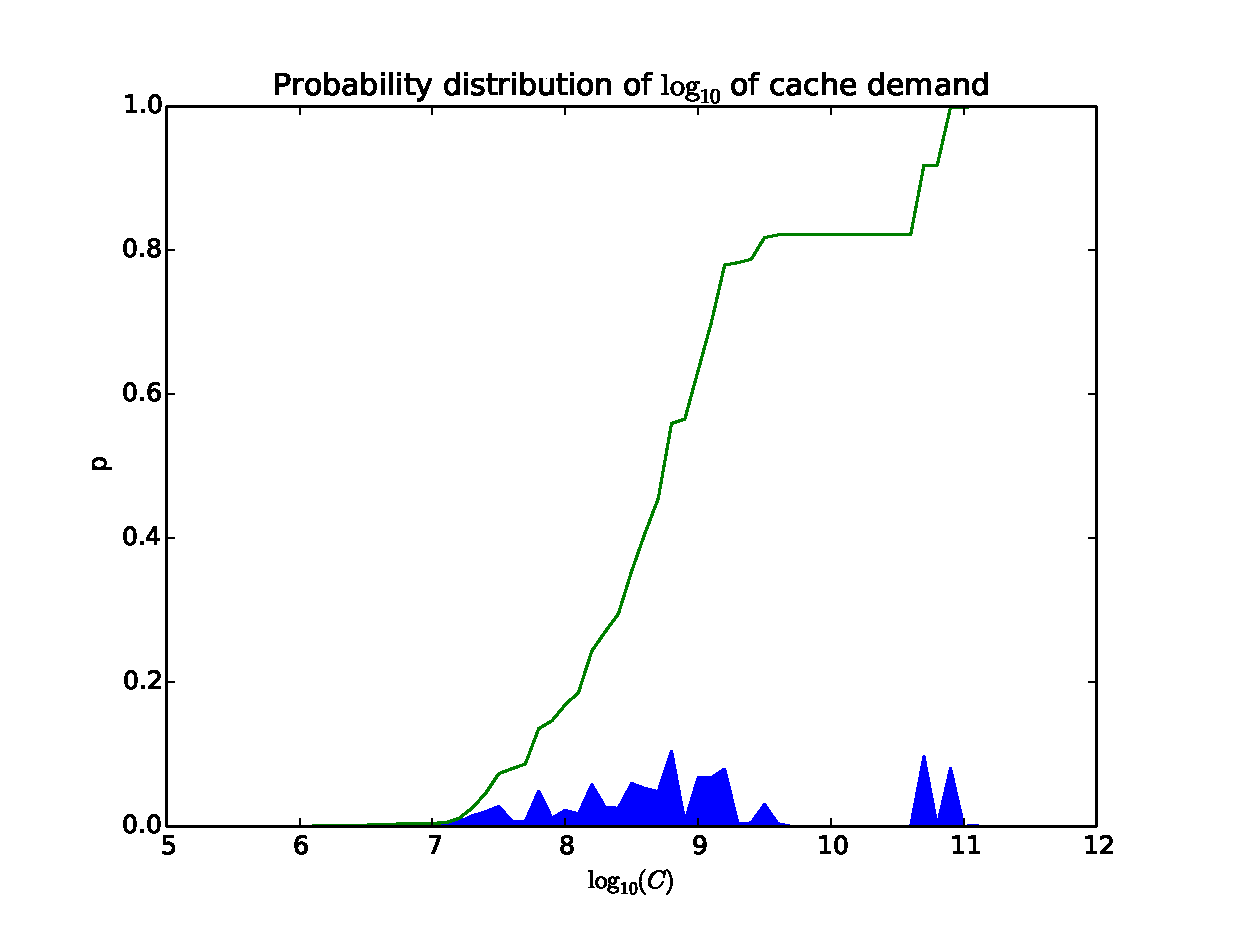
\includegraphics[width=70mm]{ocfa/step2/stripped1_virtcachesize.eps}
}
\subfloat[case 2]{
  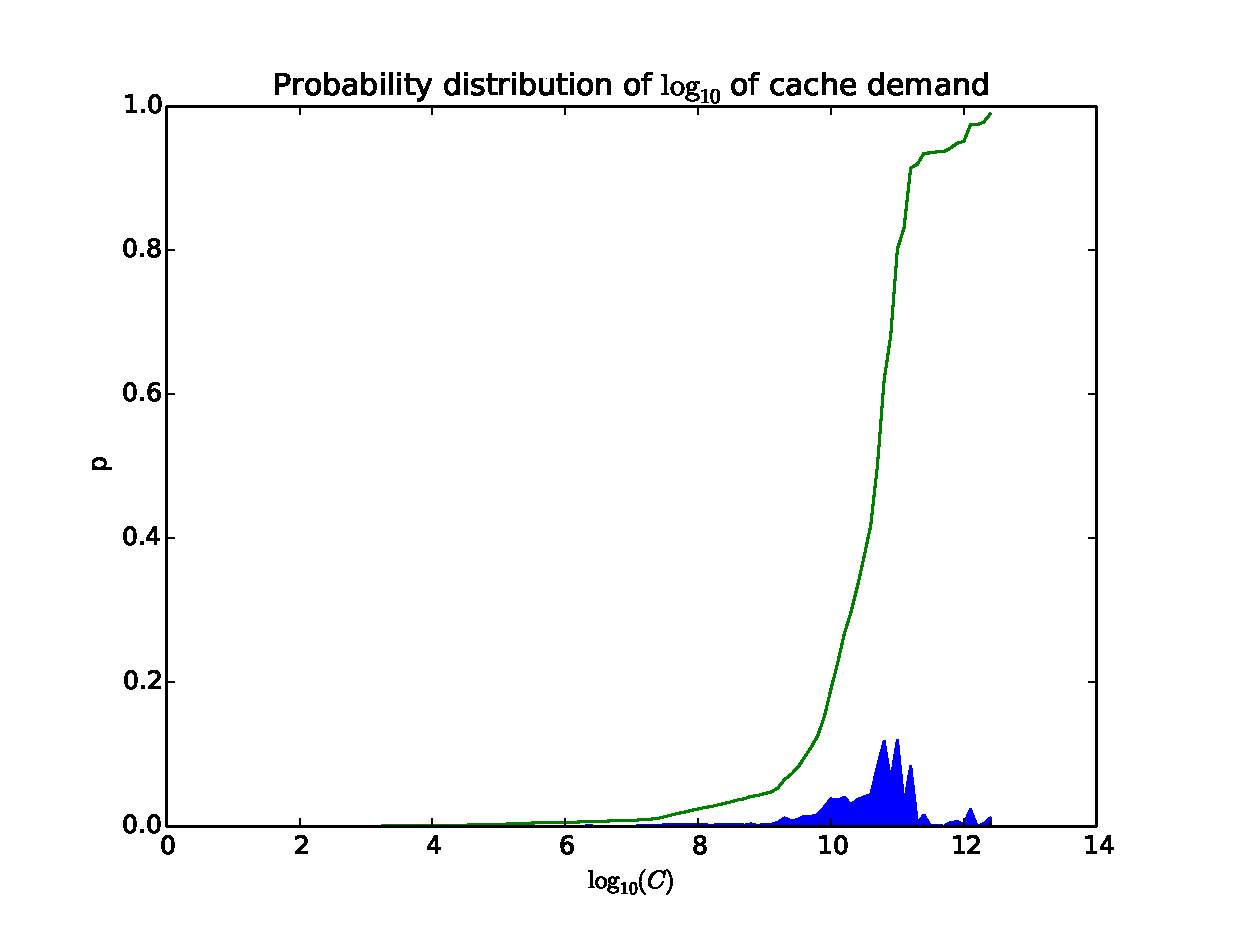
\includegraphics[width=70mm]{ocfa/step2/stripped2_virtcachesize.eps}
}
\hspace{0mm}
\subfloat[case 3]{
  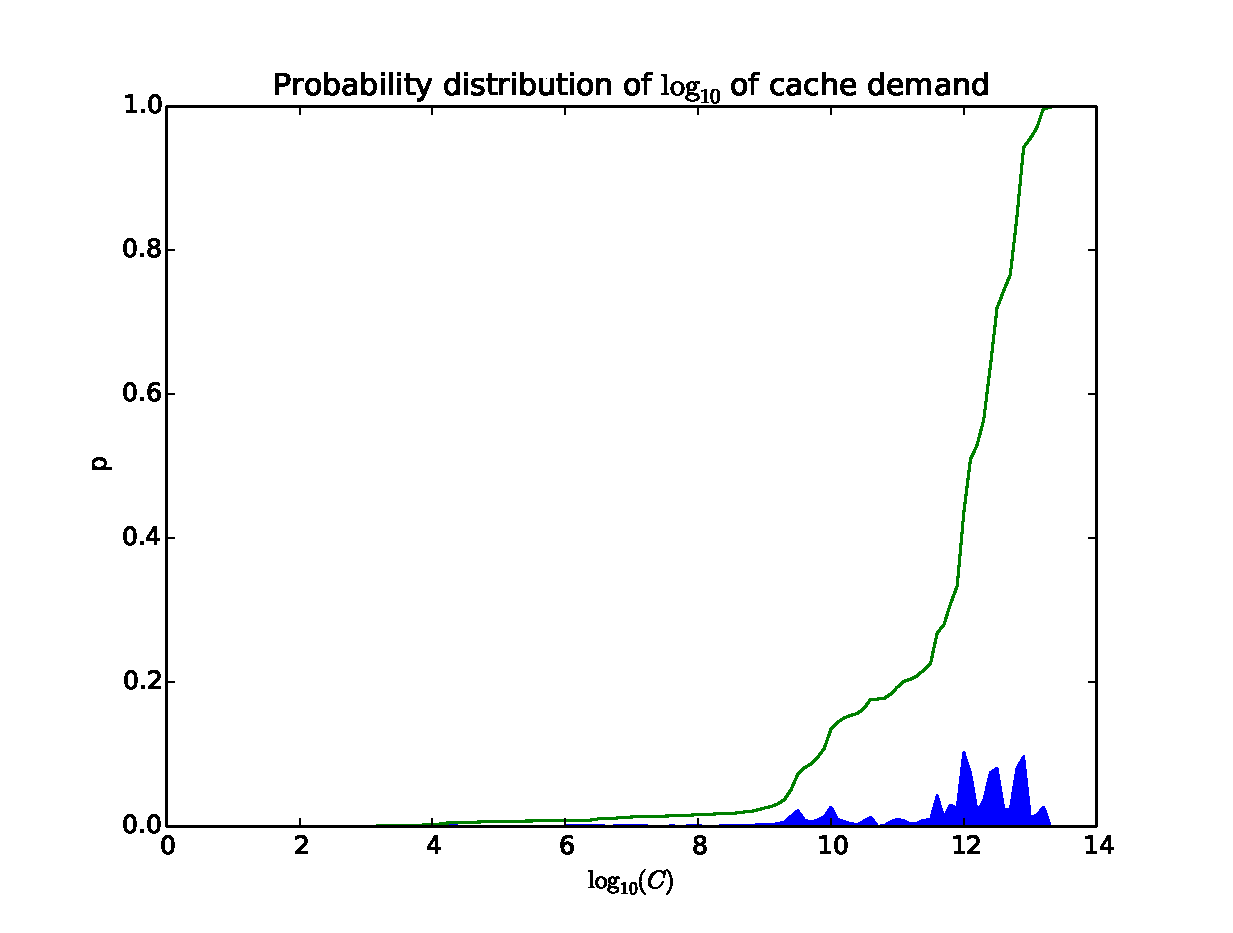
\includegraphics[width=70mm]{ocfa/step2/stripped3_virtcachesize.eps}
}
\subfloat[case 4]{
  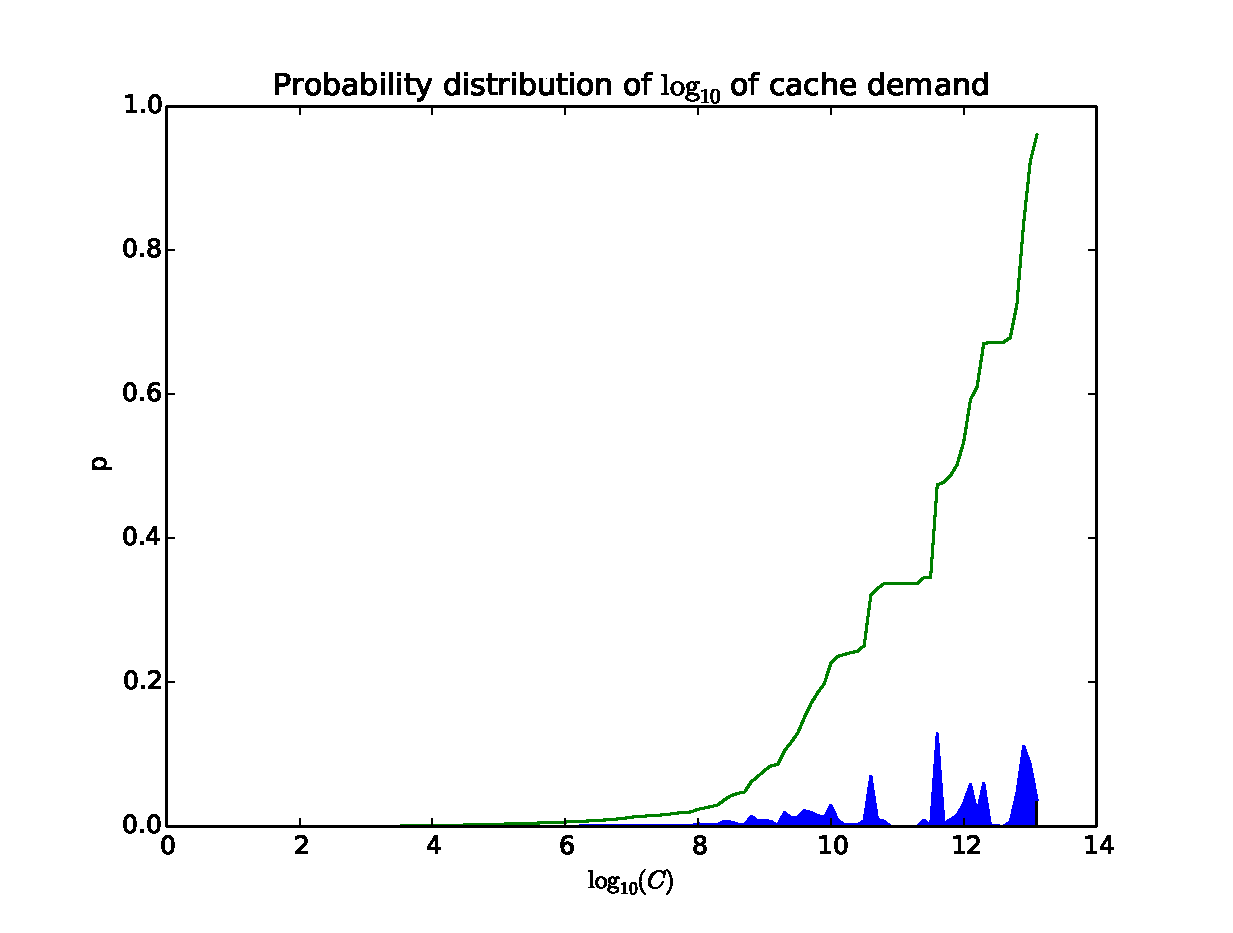
\includegraphics[width=70mm]{ocfa/step2/stripped4_virtcachesize.eps}
}
\caption{Virtual cache size probability density}
\label{fig:VirtCacheSize}
\end{figure}

\subsection{Inter-job timing}
\begin{figure}
\centering
\subfloat[case 1]{
  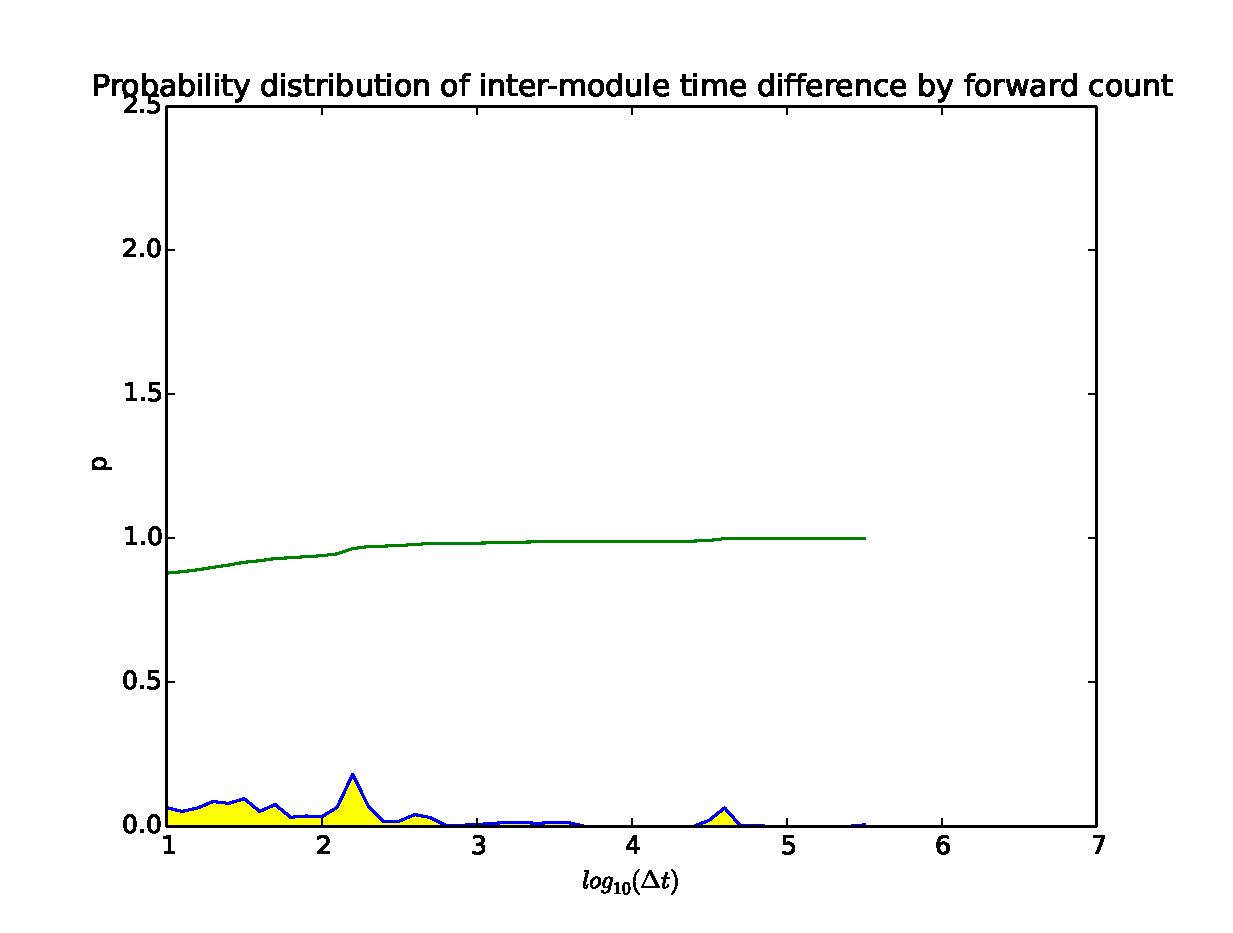
\includegraphics[width=70mm]{ocfa/step3/stripped1_prevnext_by_count.eps}
}
\subfloat[case 2]{
  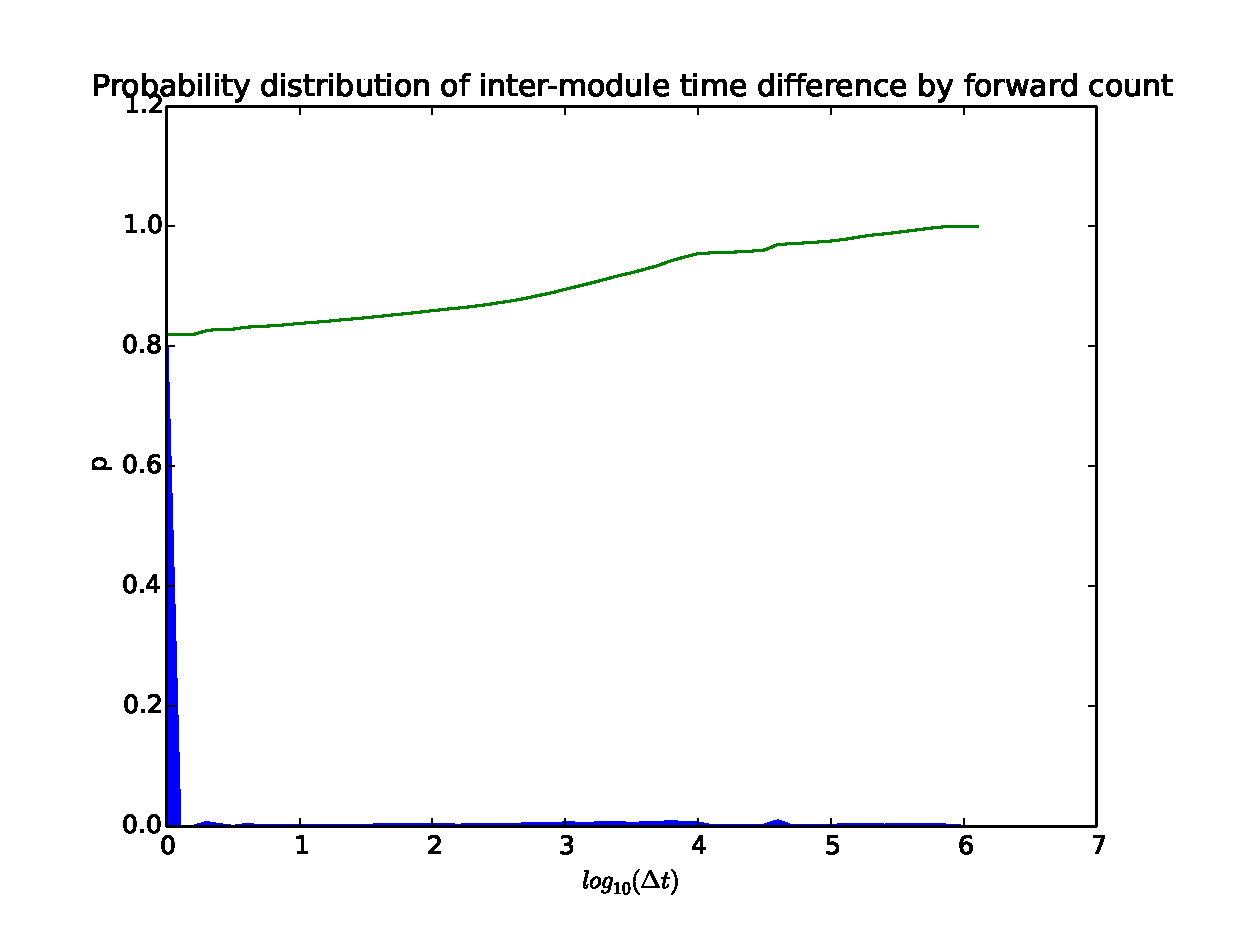
\includegraphics[width=70mm]{ocfa/step3/stripped2_prevnext_by_count.eps}
}
\hspace{0mm}
\subfloat[case 3]{
  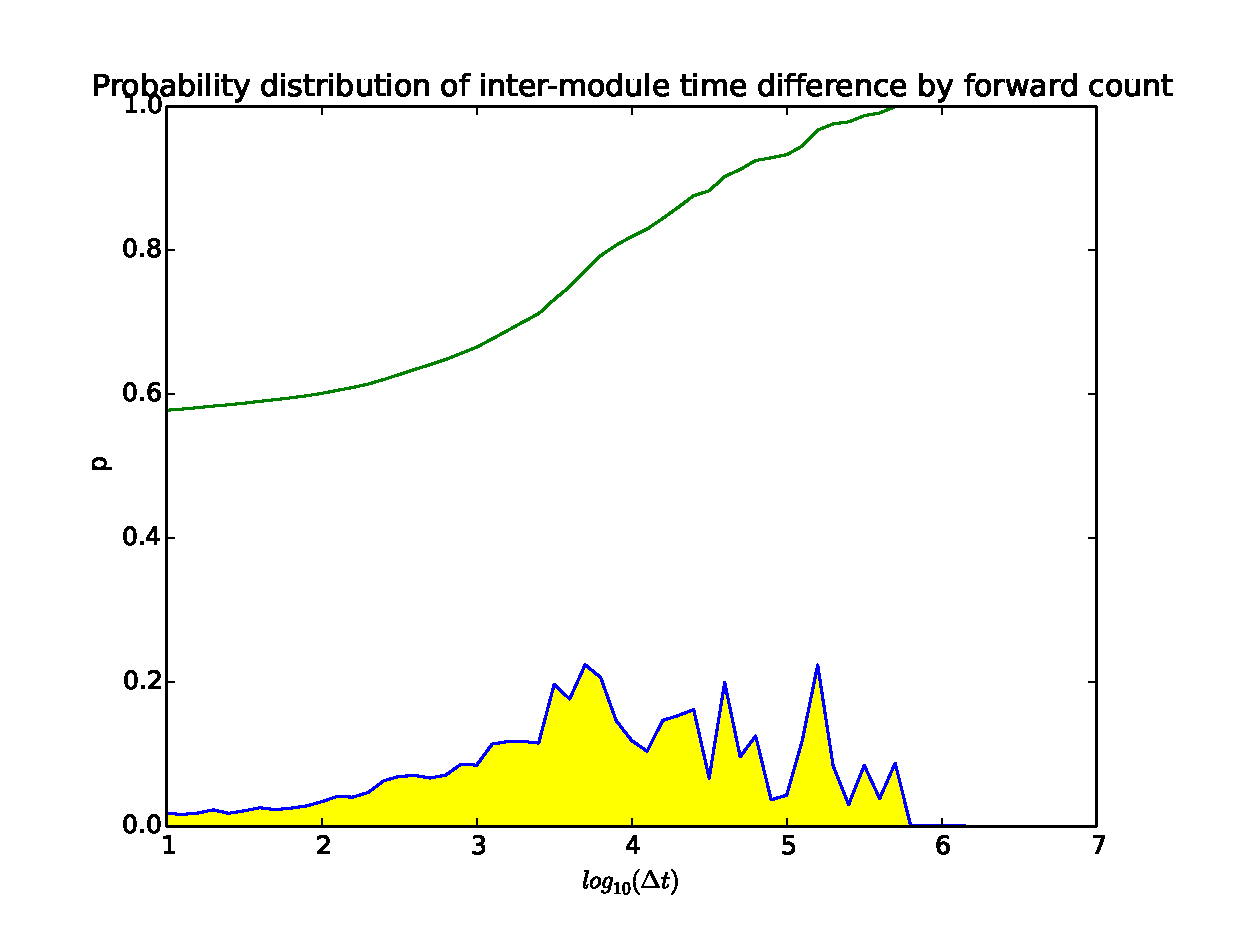
\includegraphics[width=70mm]{ocfa/step3/stripped3_prevnext_by_count.eps}
}
\subfloat[case 4]{
  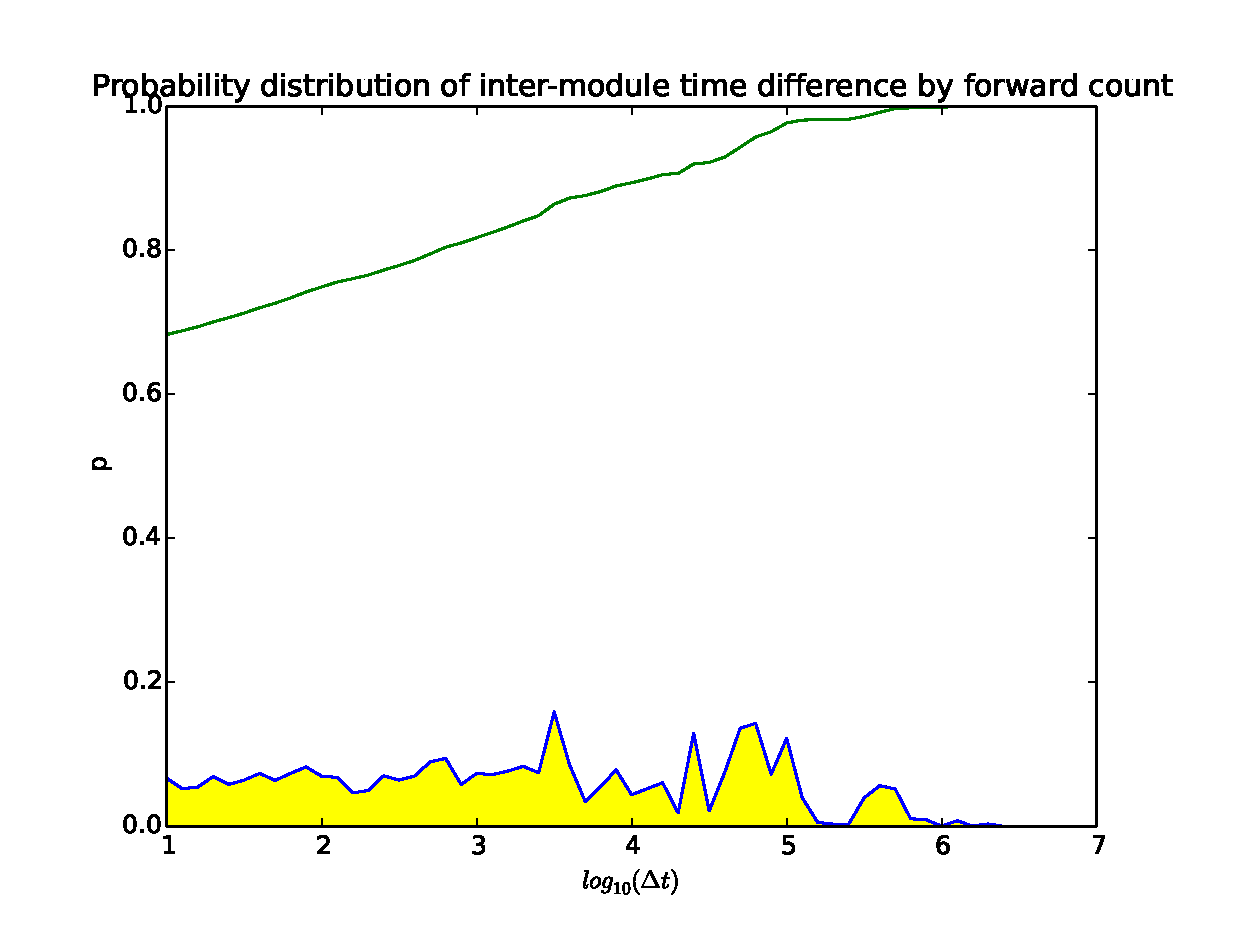
\includegraphics[width=70mm]{ocfa/step3/stripped4_prevnext_by_count.eps}
}
\caption{Inter-job time probability density}
\label{fig:InterJob}
\end{figure}
 ~\ref{fig:InterJob} on page ~\pageref{fig:Interjob} shows the probability density function of the inter-module time for modules processing the same evidence.
In the last subsection we discovered the the fact that the most of the active data would not fit in the physical memory of an OCFA server. When we look however at the probability density function of the time between two jobs, we discover that a majority of between about 60\% and 90\% of all inter-job times falls below $10^1$ seconds mark. While there are times extending up to and exceeding the $10^6$ seconds visible in some of the graphs, most of the inter-module times are so small in comparison that disk cache hits would seem almost inevitable. These results are quite inconclusive so far, so we need to look at other results still.
\subsection{Inter-job timing by content size}
\begin{figure}
\centering
\subfloat[case 1]{
  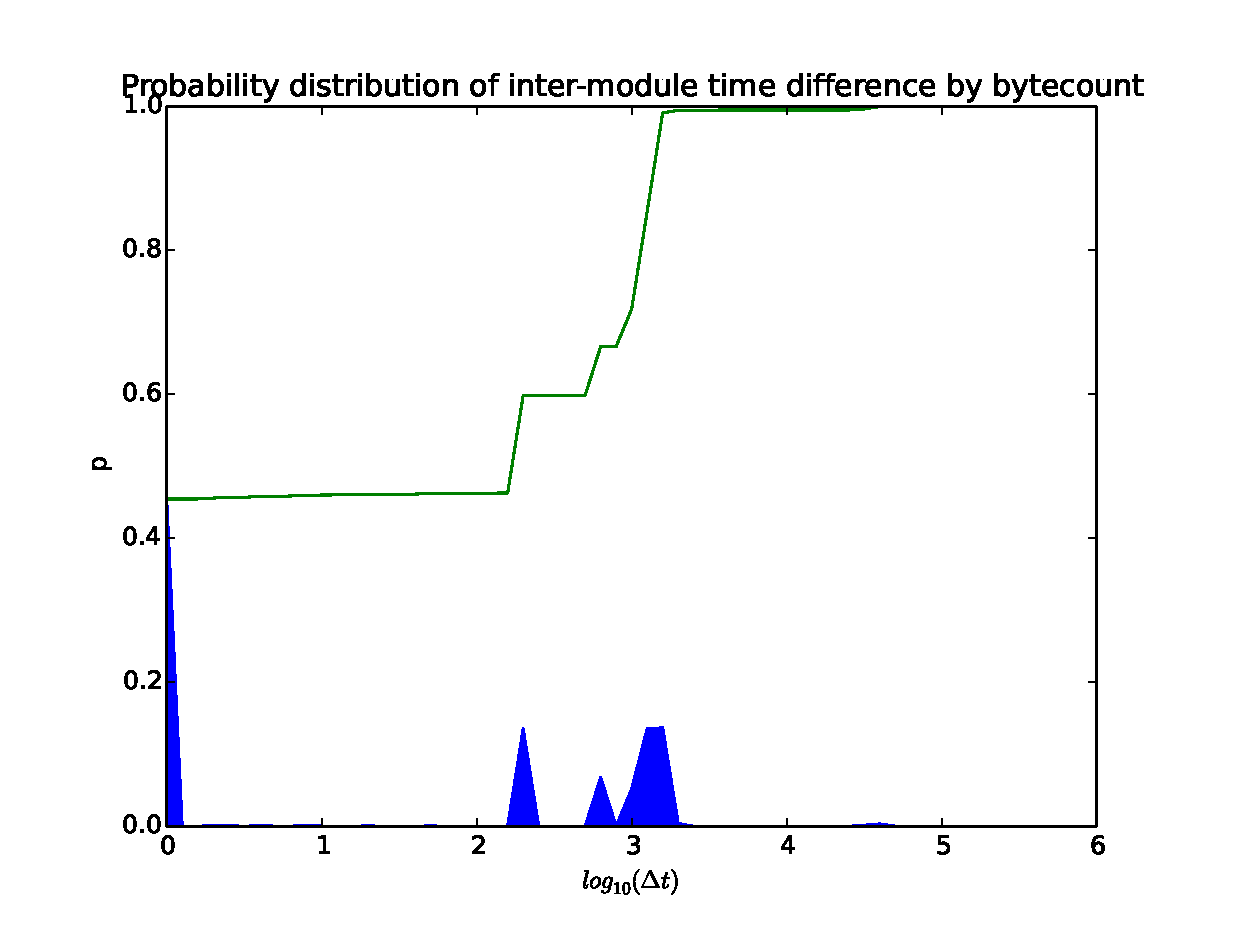
\includegraphics[width=70mm]{ocfa/step3/stripped1_prevnext_by_size.eps}
}
\subfloat[case 2]{
  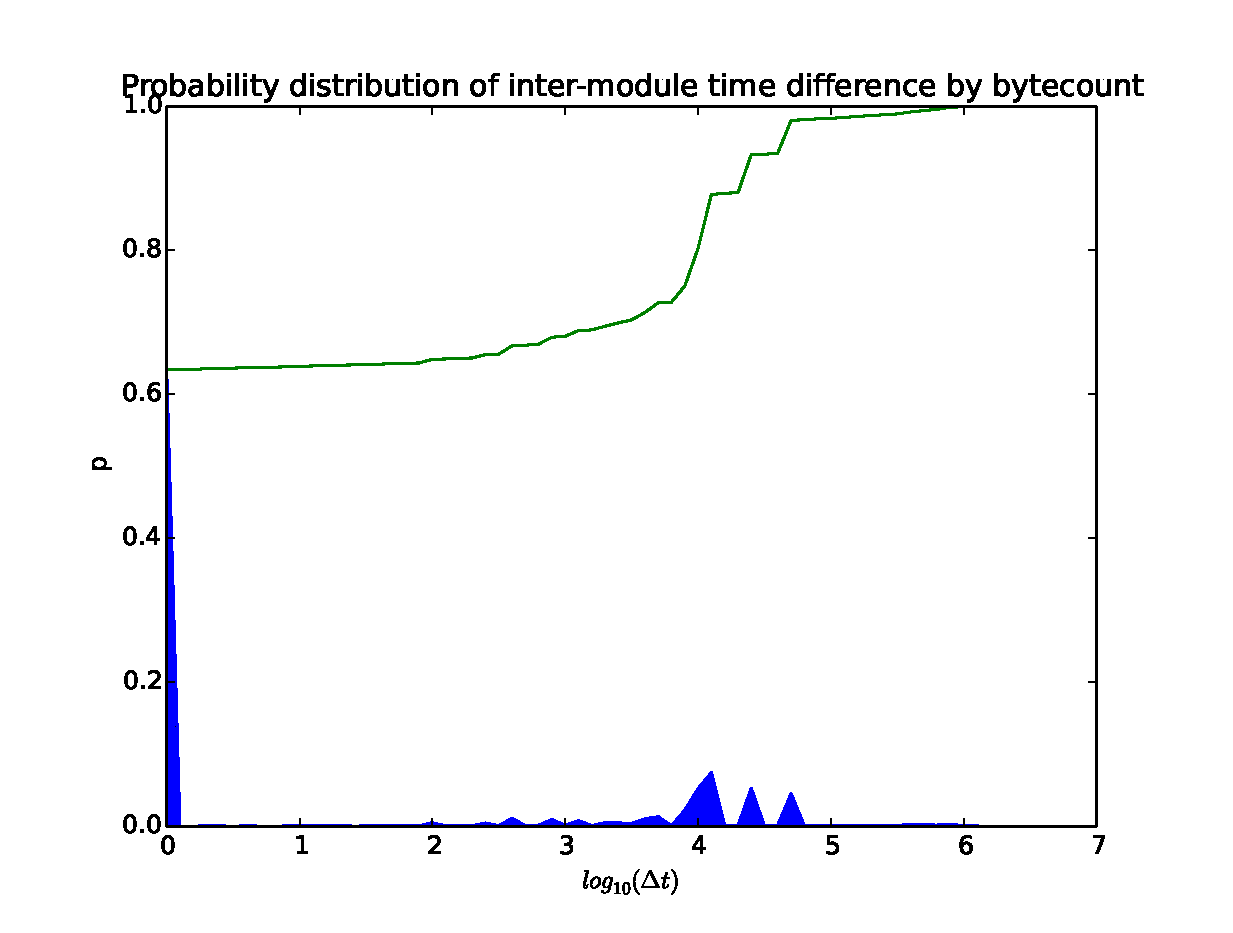
\includegraphics[width=70mm]{ocfa/step3/stripped2_prevnext_by_size.eps}
}
\hspace{0mm}
\subfloat[case 3]{
  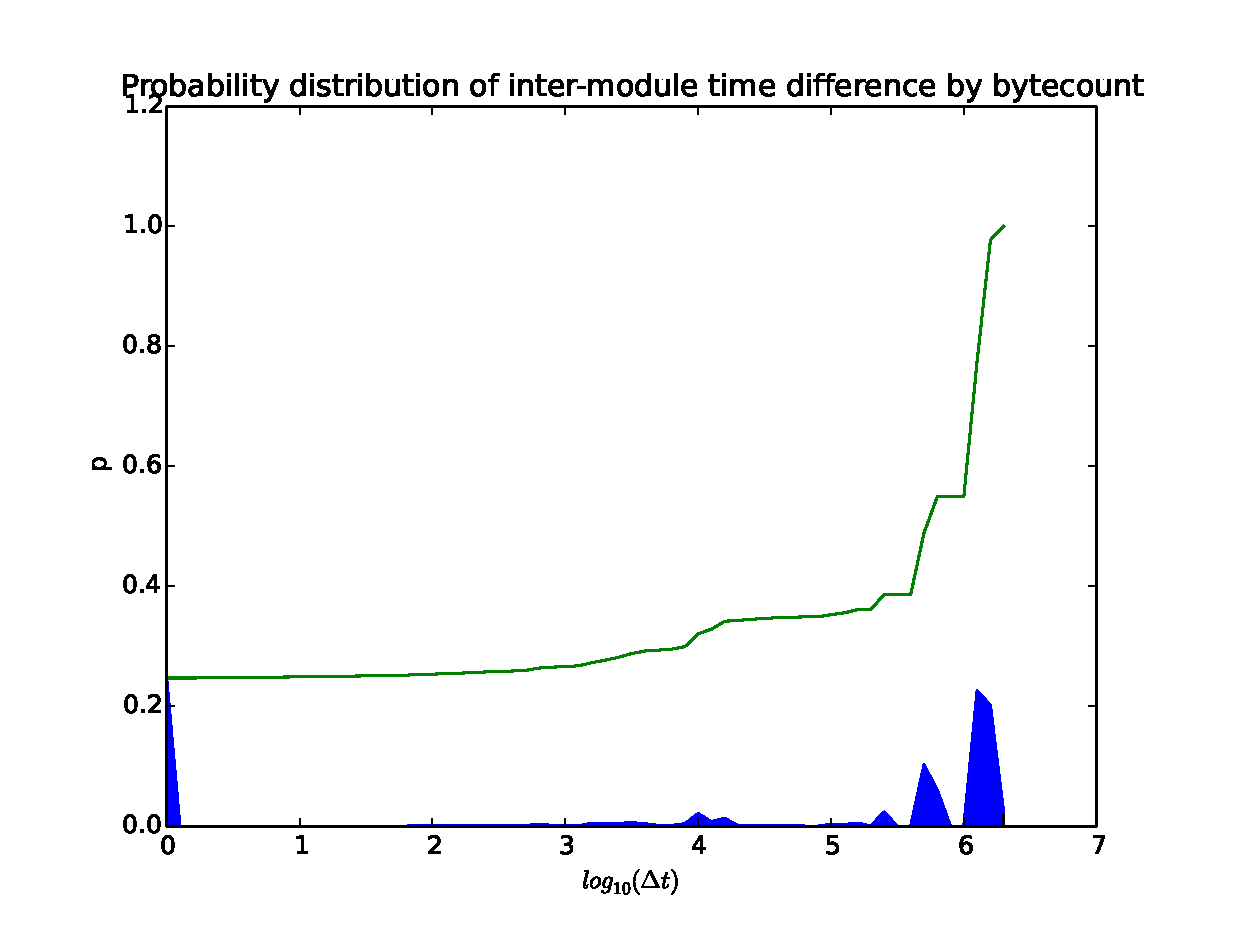
\includegraphics[width=70mm]{ocfa/step3/stripped3_prevnext_by_size.eps}
}
\subfloat[case 4]{
  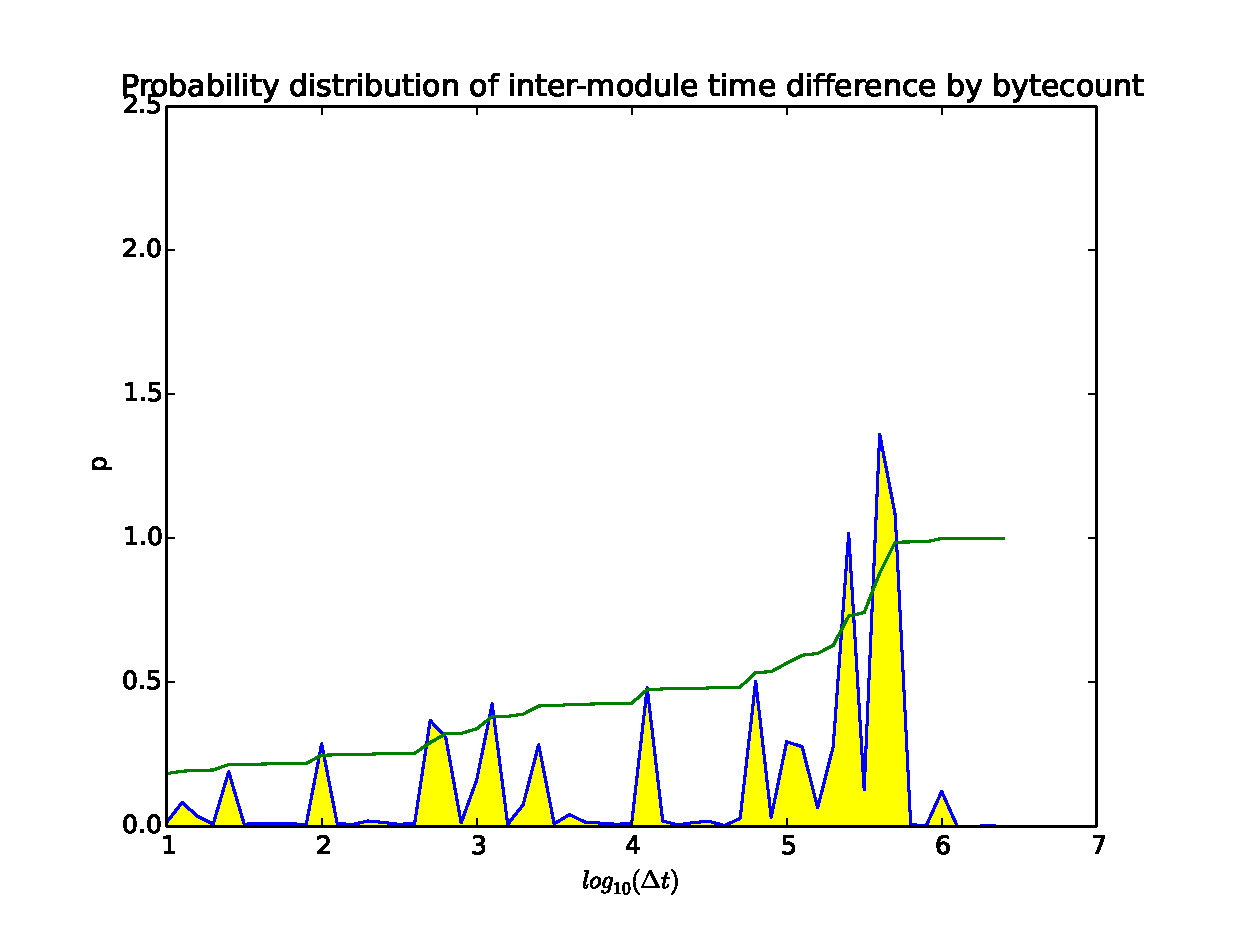
\includegraphics[width=70mm]{ocfa/step3/stripped4_prevnext_by_size.eps}
}
\caption{Inter-job time probability density by volume}
\label{fig:InterJobBySize}
\end{figure}
If instead of weighing the probability density function by the number data events, we weigh it by the amount of data, the picture that we saw in the previous subsection shifts significantly. ~\ref{fig:InterJobBySize} on page ~\pageref{fig:InterjobBySize} shows this shift. A relatively large portion of the data now shows to have a job time interval of well over $10^4$ seconds. That means multiple hours, long enough to expect any disk caching to long have been overwritten so that a consecutive read would surely lead to a disk-cache miss.
\subsection{First-last timing}
\begin{figure}
\centering
\subfloat[case 1]{
  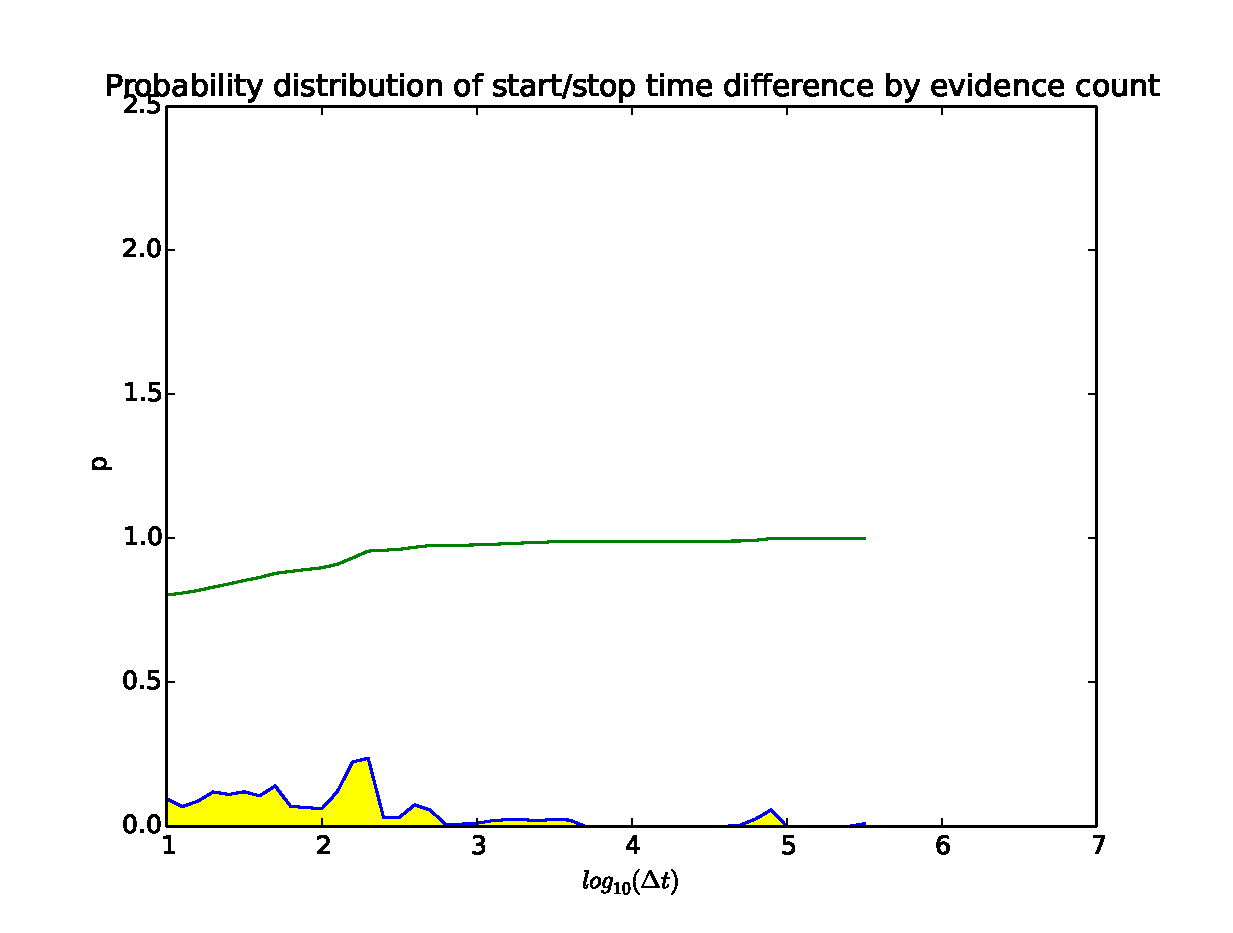
\includegraphics[width=70mm]{ocfa/step3/stripped1_startstop_by_count.eps}
}
\subfloat[case 2]{
  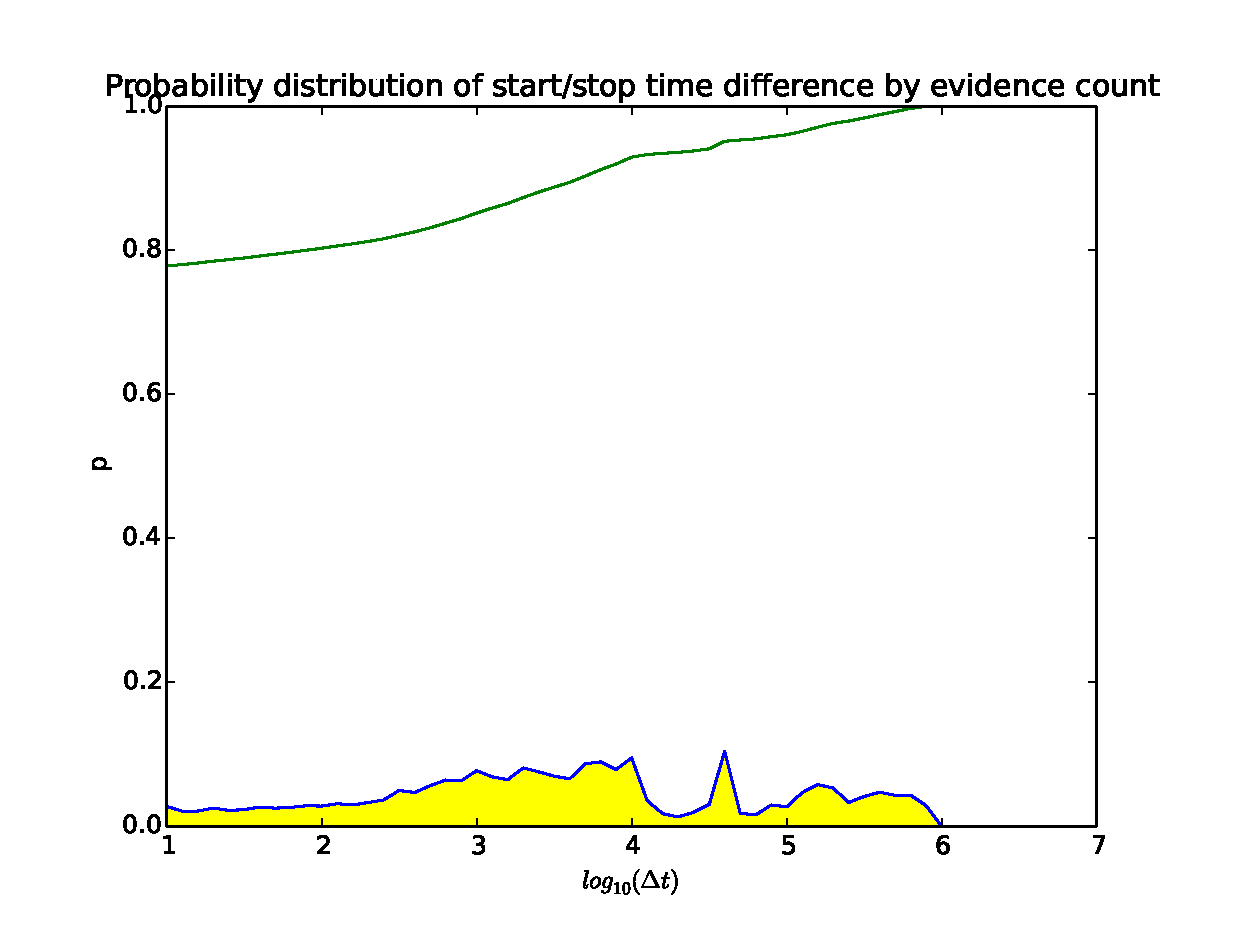
\includegraphics[width=70mm]{ocfa/step3/stripped2_startstop_by_count.eps}
}
\hspace{0mm}
\subfloat[case 3]{
  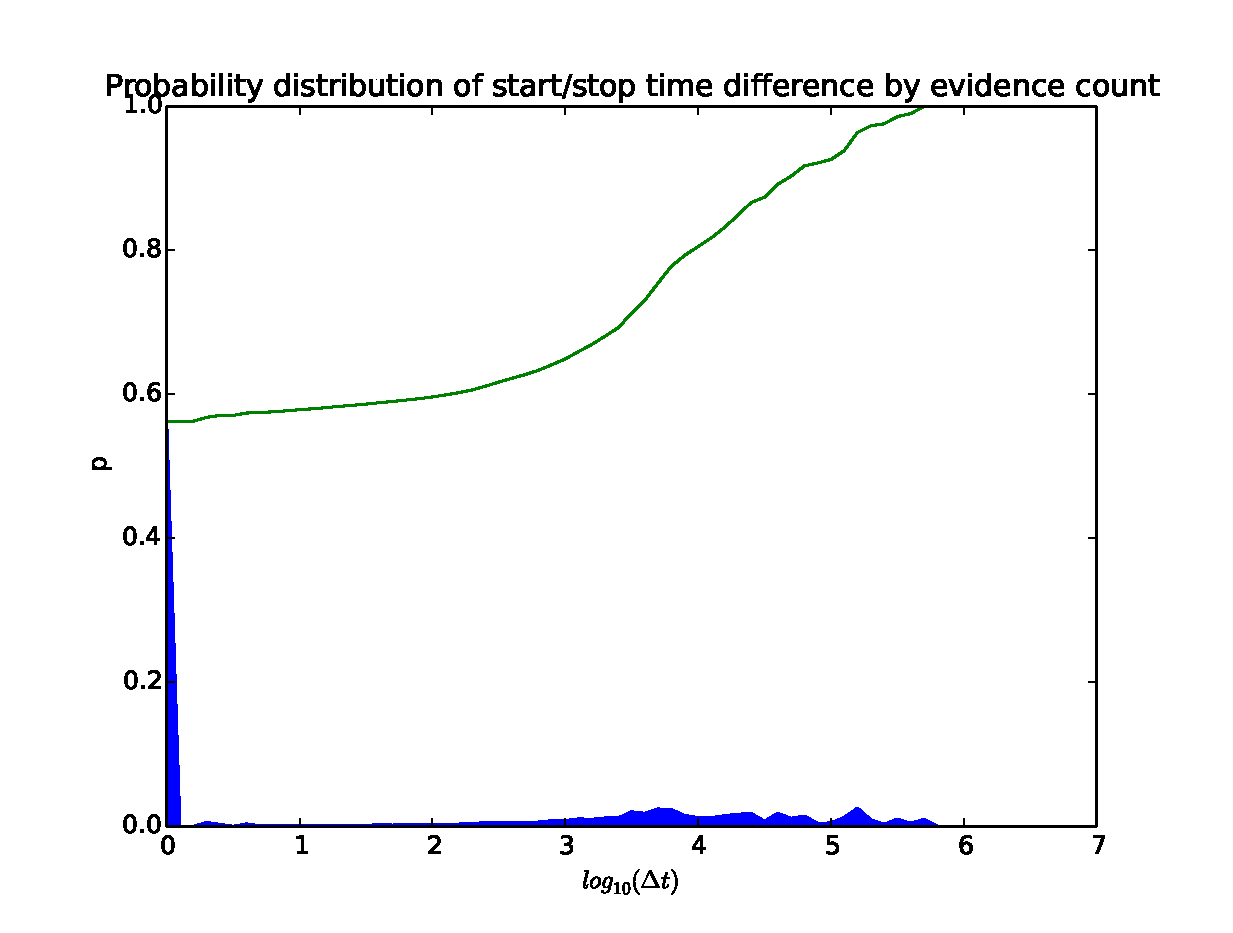
\includegraphics[width=70mm]{ocfa/step3/stripped3_startstop_by_count.eps}
}
\subfloat[case 4]{
  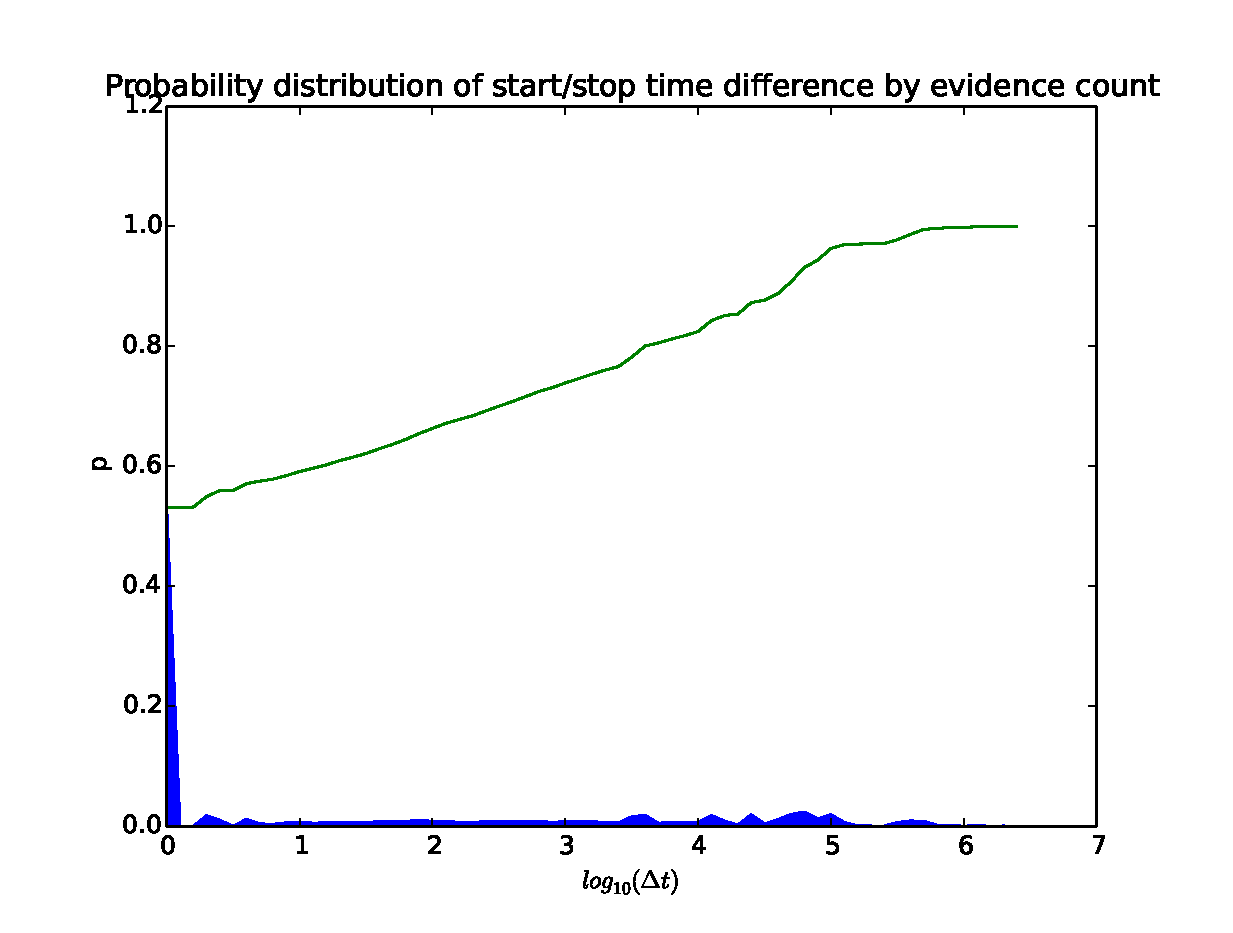
\includegraphics[width=70mm]{ocfa/step3/stripped4_startstop_by_count.eps}
}
\caption{First-last time probability density}
\label{fig:FirstLast}
\end{figure}
Given that our inter-job timing stats were inconclusive, we look at the timing interval between the first module creating the data entity and the last data processing module being done with it. In ~\ref{fig:FirstLast} on page ~\pageref{fig:FirstLast} we see that while less expressed than for ~\pageref{fig:Interjob}, still fast a majority of about 60\% to 80\% of evidences will be completely done in less than ten seconds. these results while being in line with our expectations for the OCFA priority system, still don't match the other results we have seen so far.
\subsection{First-last timing by content size}
\begin{figure}
\centering
\subfloat[case 1]{
  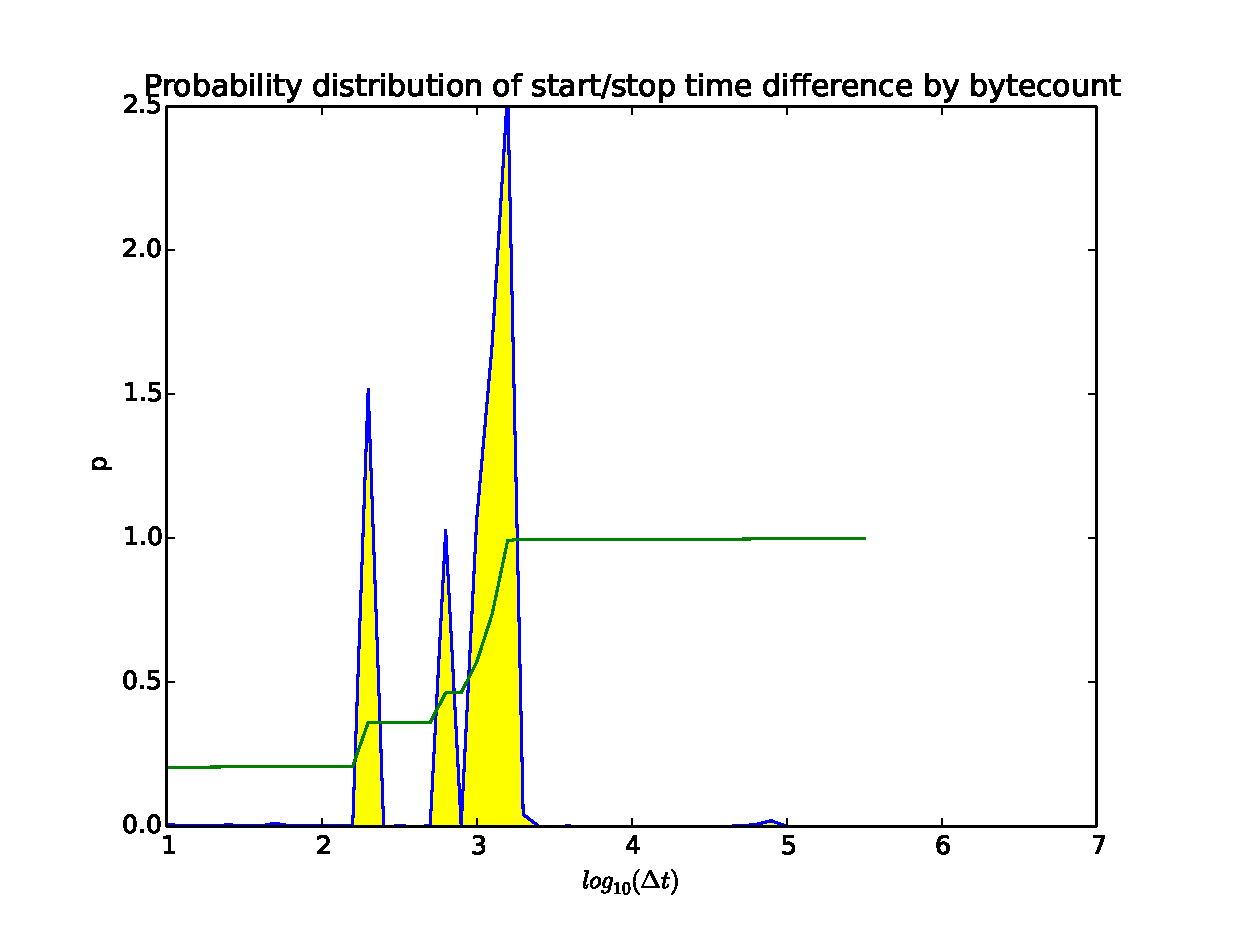
\includegraphics[width=70mm]{ocfa/step3/stripped1_startstop_by_size.eps}
}
\subfloat[case 2]{
  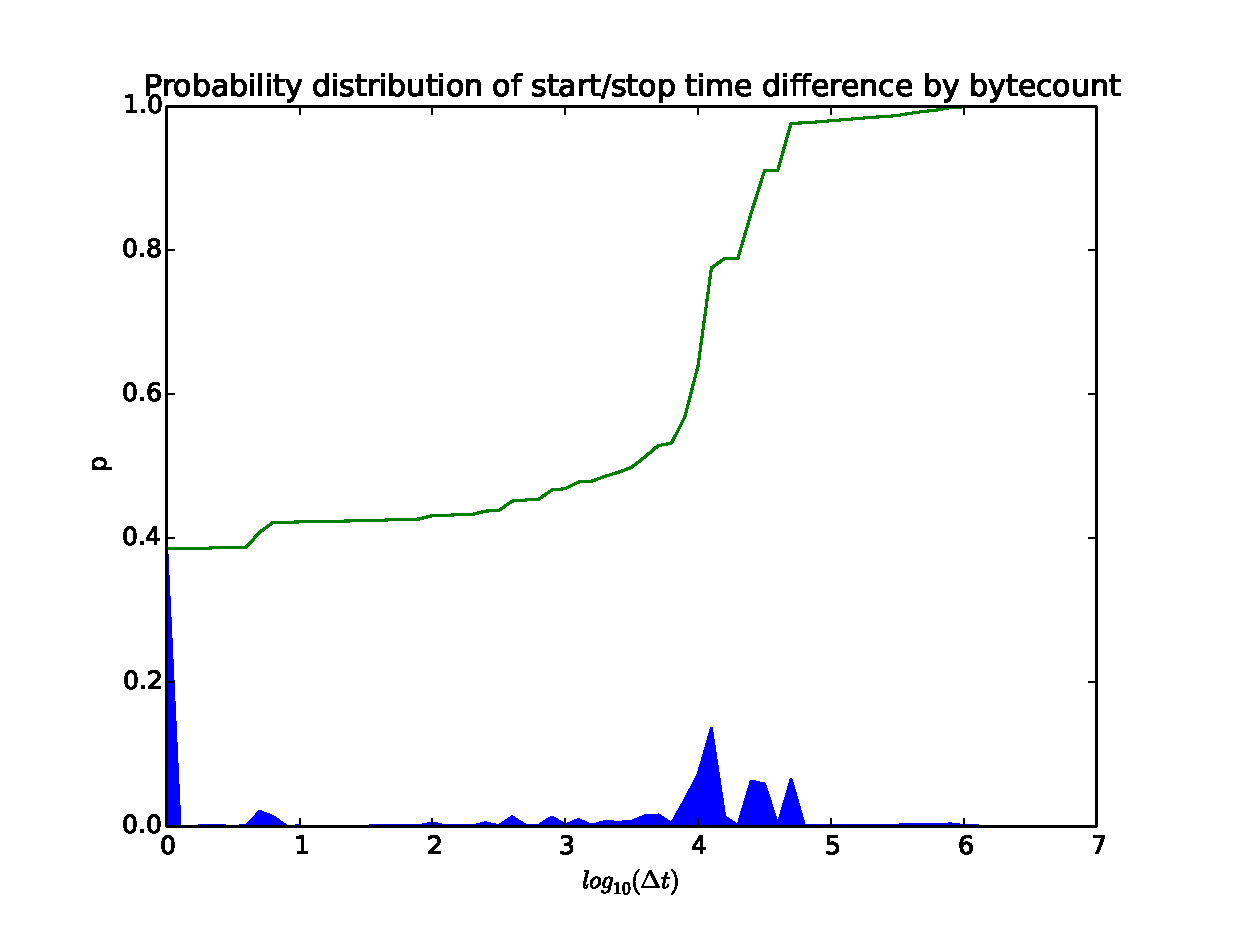
\includegraphics[width=70mm]{ocfa/step3/stripped2_startstop_by_size.eps}
}
\hspace{0mm}
\subfloat[case 3]{
  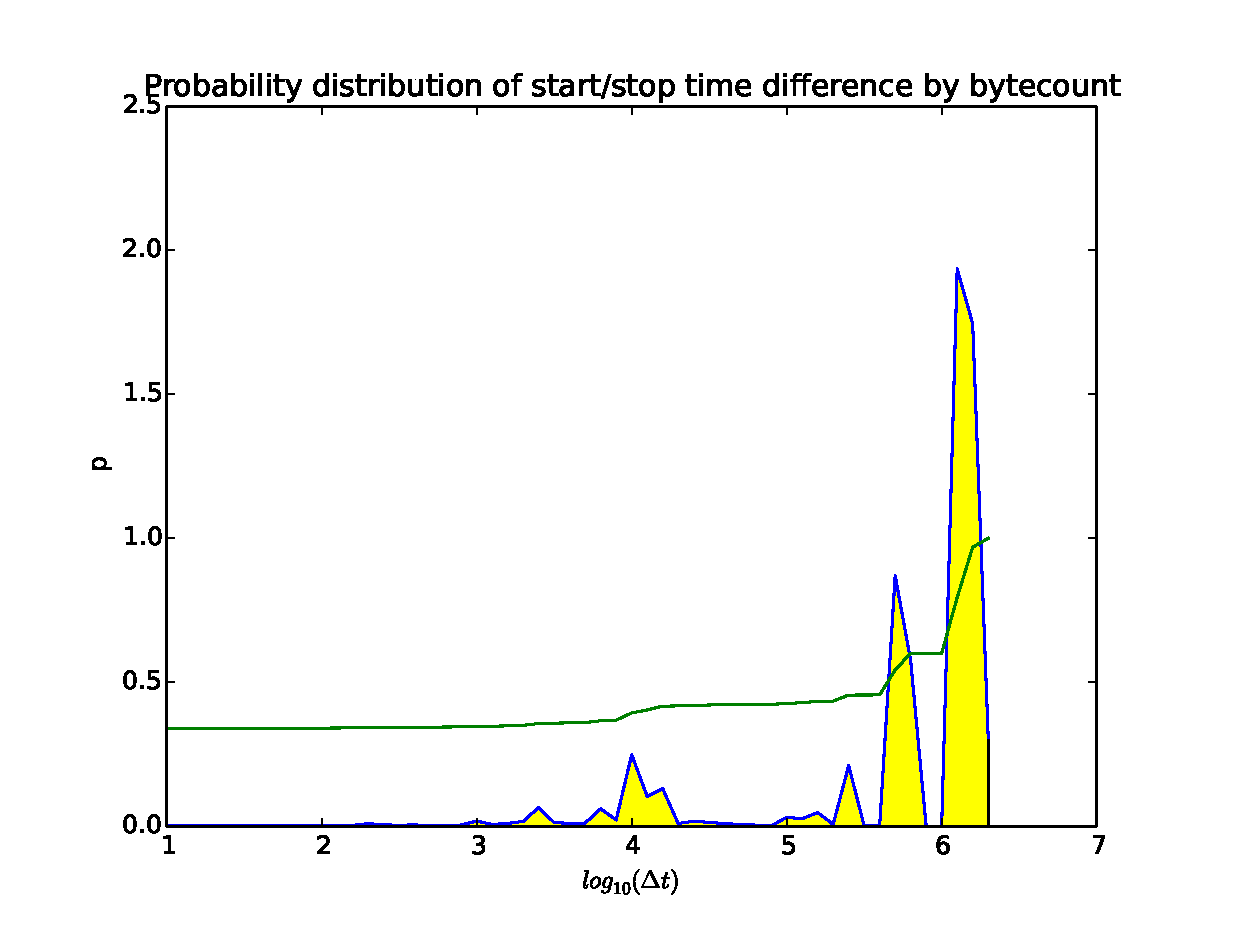
\includegraphics[width=70mm]{ocfa/step3/stripped3_startstop_by_size.eps}
}
\subfloat[case 4]{
  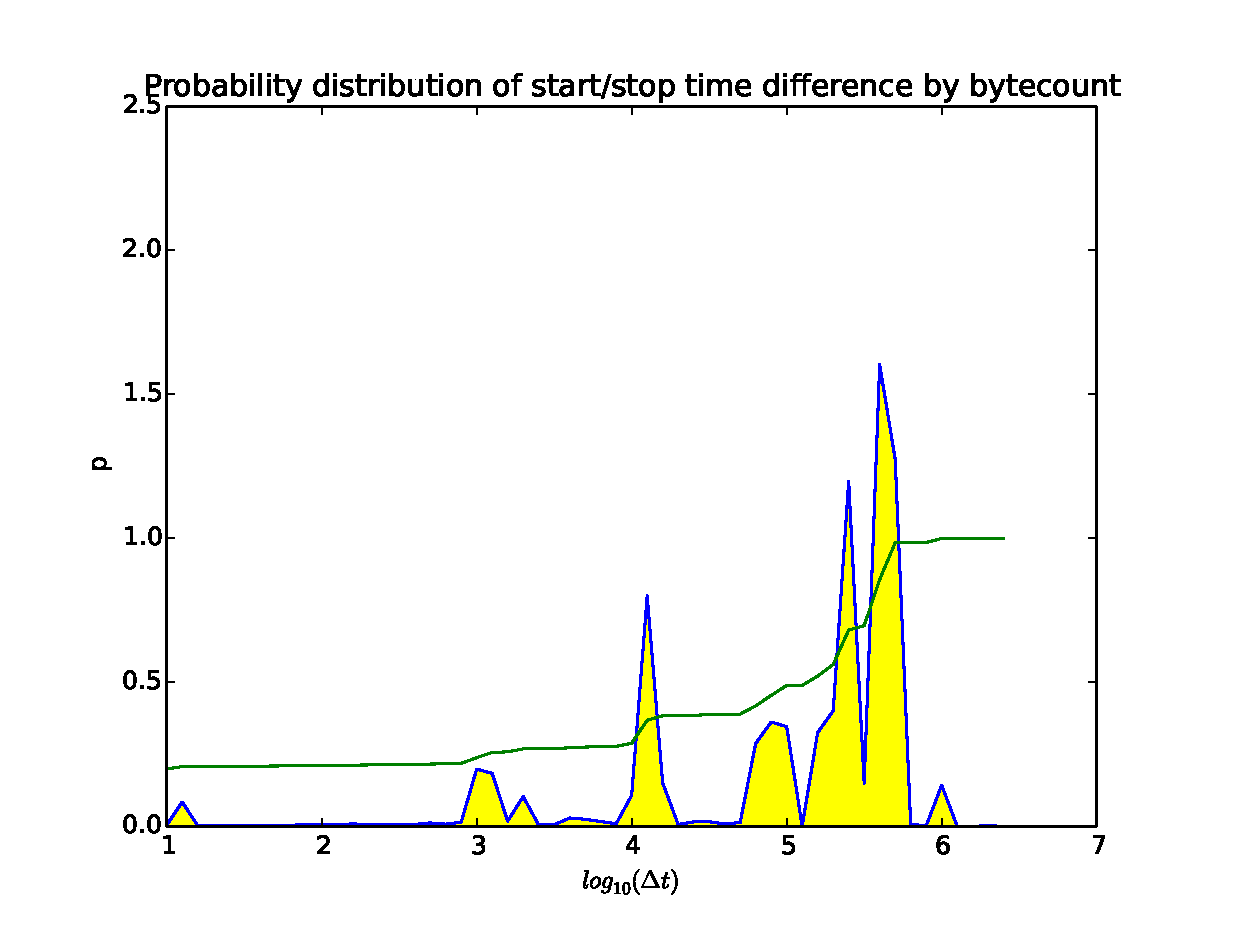
\includegraphics[width=70mm]{ocfa/step3/stripped4_startstop_by_size.eps}
}
\caption{First-last time probability density by volume}
\label{fig:FirstLastiBySize}
\end{figure}

In ~\ref{fig:FirstLastBySize} on page ~\pageref{fig:FirstLastBySize} we see the pattern we saw earlier in ~\ref{fig:InterJobBySize}, yet much more expressed. In most of the four investigations, a majority of the data will take multiple hours to get from the first module to touch/produce it to the last module to process its data. This is again a clear sign that we can expect a whole lot of disk cache misses during the lifetime of a piece of larger data within the OCFA system.

\subsection{Inflow and outflow for our fictitious cache}
\begin{figure}
\centering
\subfloat[case 1]{
  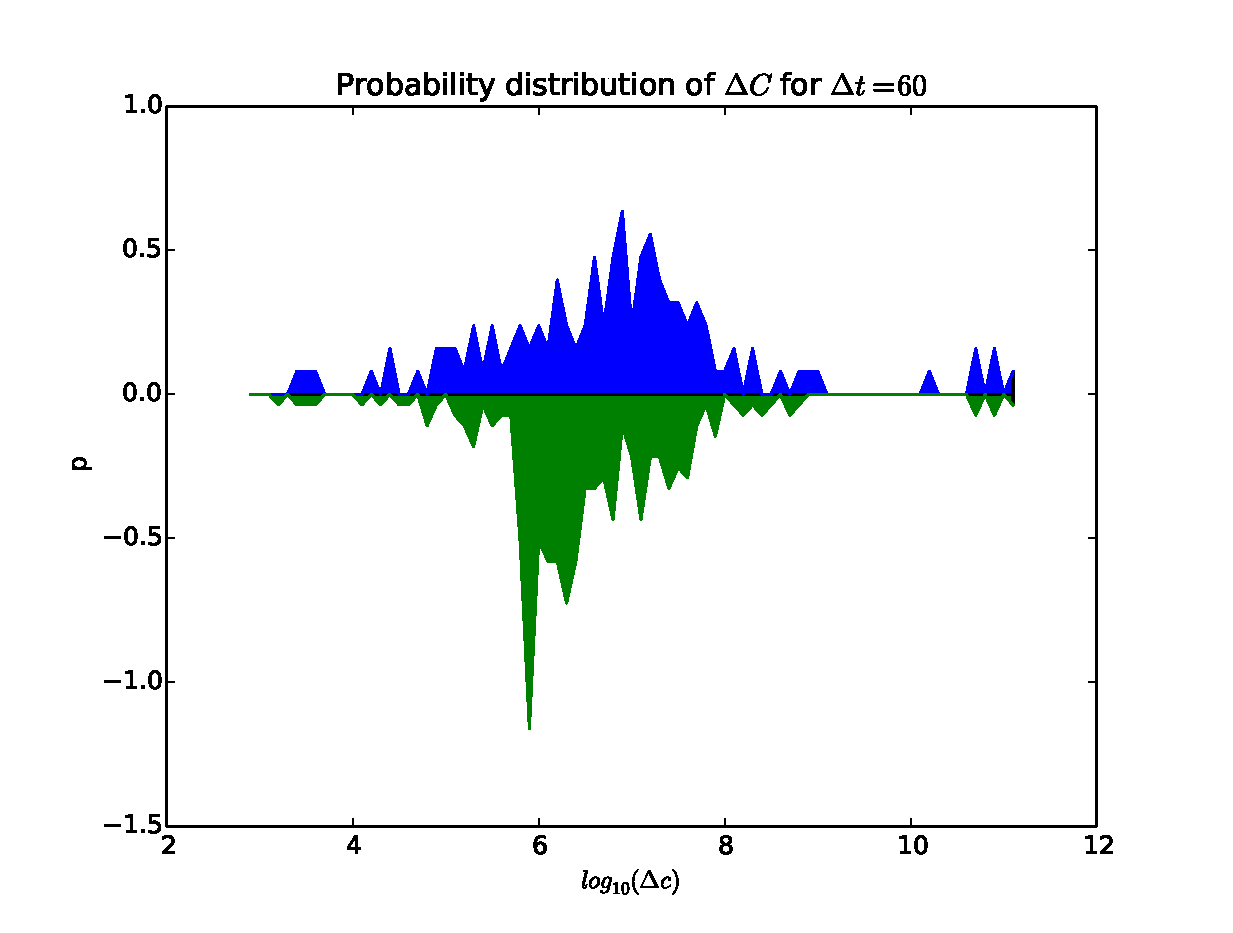
\includegraphics[width=70mm]{ocfa/step4/stripped1_inflow.eps}
}
\subfloat[case 2]{
  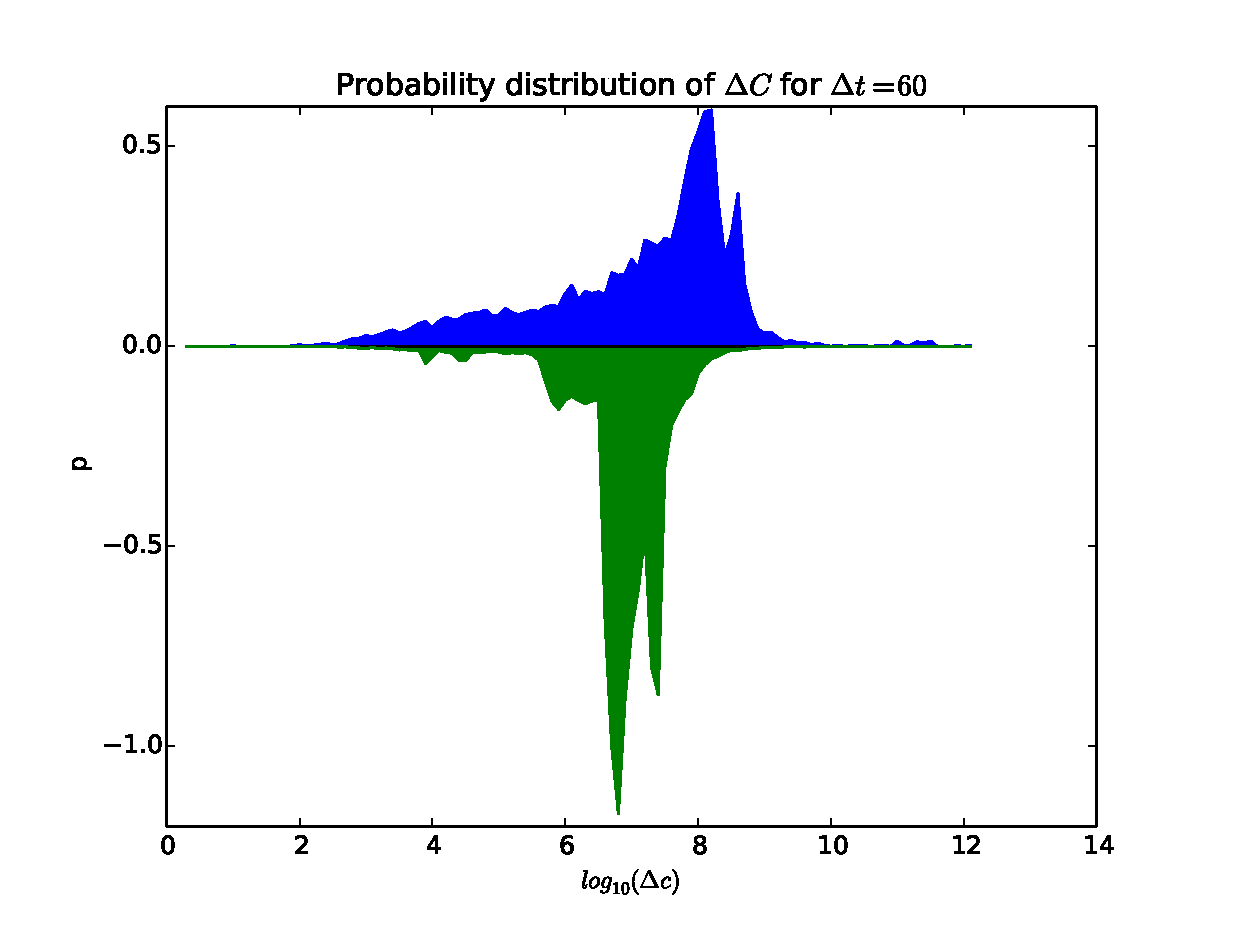
\includegraphics[width=70mm]{ocfa/step4/stripped2_inflow.eps}
}
\hspace{0mm}
\subfloat[case 3]{
  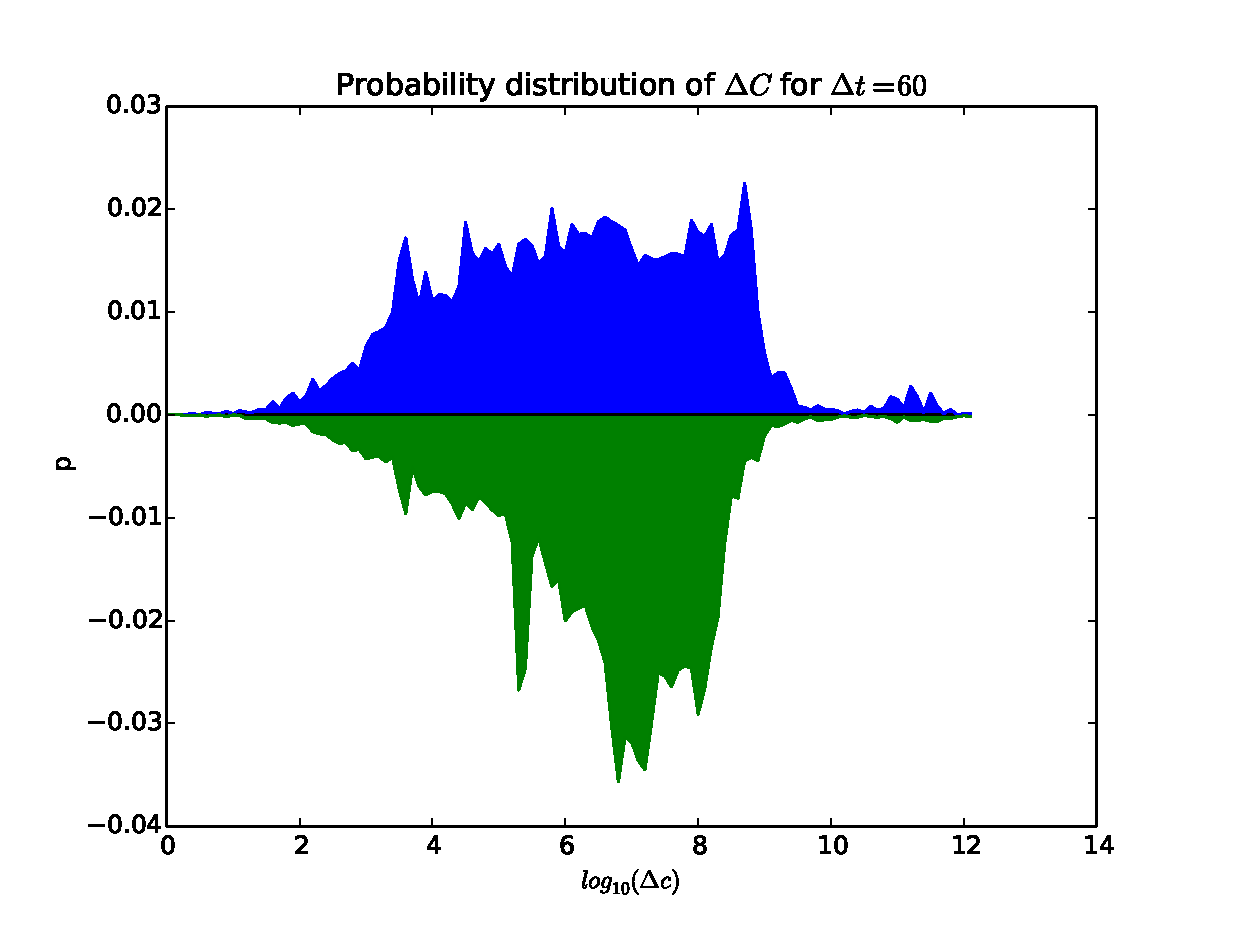
\includegraphics[width=70mm]{ocfa/step4/stripped3_inflow.eps}
}
\subfloat[case 4]{
  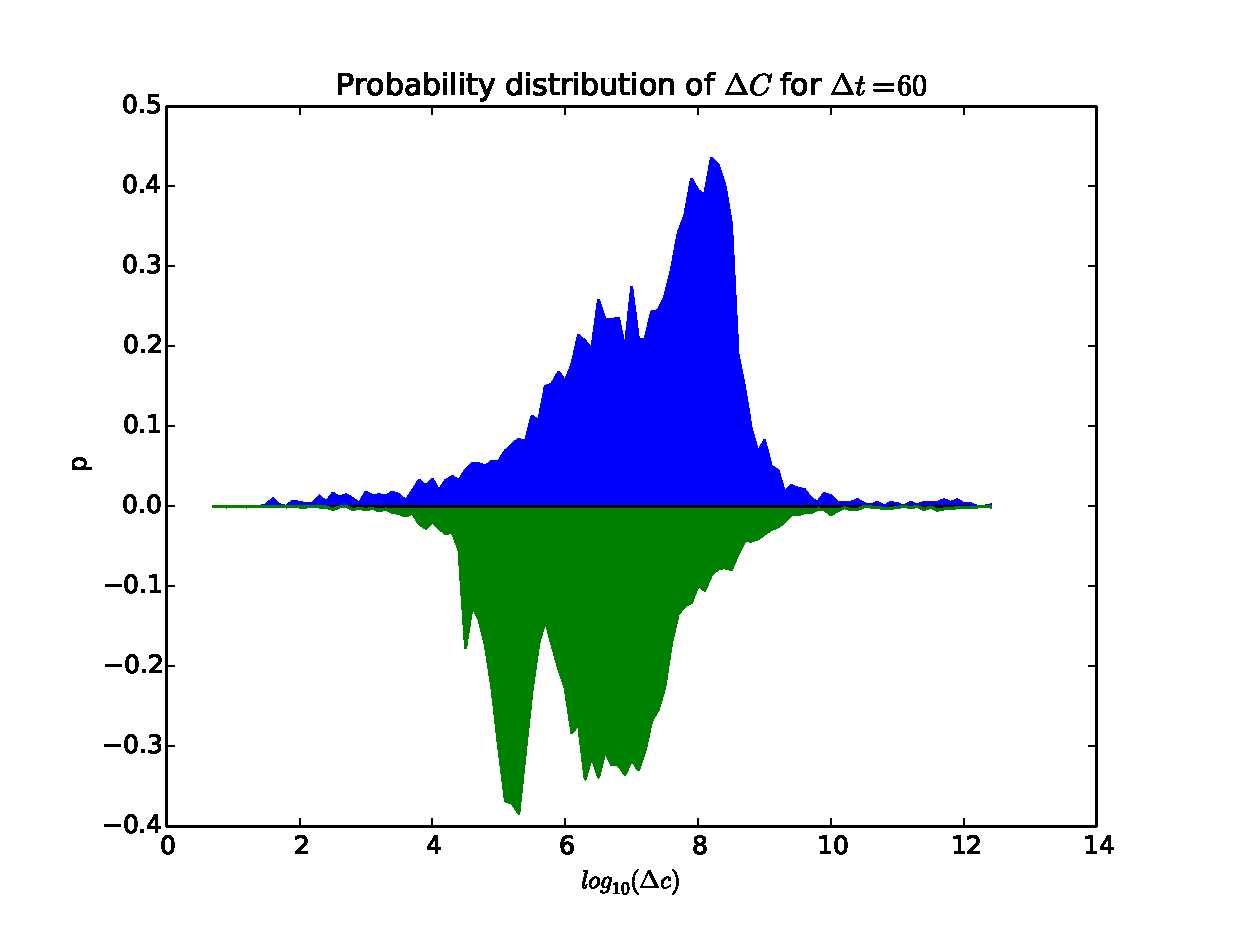
\includegraphics[width=70mm]{ocfa/step4/stripped4_inflow.eps}
}
\caption{In/out flow probability density}
\label{fig:FlowInOut}
\end{figure}
The pictures in ~\ref{fig:FlowInOut} on page ~\pageref{fig:FlowInOut} finally shows the problem with the disk cache misses. It shows both the probability density of growth of the amount of \emph{active} data in the system, and on the negative axis the probability density of shrinkage in one minute intervals. If we remember that this density function is plotted on a logarithmic X, we can identify that the growth density on the upper end of the graphs is higher than the shrinkage density on the upper end of the graph. This means that while there may be many minutes where there is significant shrinkage, the over time amount of \emph{active} data will grow as new data continues being submitted to the system. These results show a clearly that for the OCFA system, there is an imbalance between the data input speed and the overall data processing speed. With knowledge about the investigation, we can further see that the significant production of new evidence data events by modules other than the Java based kickstart, significantly increases the visual noticeable imbalance in these graphs for case two and four.  

\section{Inter-module flows}
FIXME: we need text here.
\begin{figure}
  \centering
  \includegraphics[width=130mm]{ocfa/step5/stripped1_modules.eps}
  \caption{Case 1 inter-module flows}
\end{figure}
\begin{figure}
  \centering
  \includegraphics[width=130mm]{ocfa/step5/stripped2_modules.eps}
  \caption{Case 2 inter-module flows}
\end{figure}
\begin{figure}
  \centering
  \includegraphics[width=130mm]{ocfa/step5/stripped3_modules.eps}
  \caption{Case 3 inter-module flows}
\end{figure}
\begin{figure}
  \centering
  \includegraphics[width=130mm]{ocfa/step5/stripped4_modules.eps}
  \caption{Case 4 inter-module flows}
\end{figure}
\begin{figure}
\centering
\subfloat[case 1]{
  \includegraphics[width=70mm]{ocfa/step5/stripped1_modtypes.eps}
}
\subfloat[case 2]{
  \includegraphics[width=70mm]{ocfa/step5/stripped2_modtypes.eps}
}
\hspace{0mm}
\subfloat[case 3]{
  \includegraphics[width=70mm]{ocfa/step5/stripped3_modtypes.eps}
}
\subfloat[case 4]{
  \includegraphics[width=70mm]{ocfa/step5/stripped4_modtypes.eps}
}
\caption{Rough data flow}
\end{figure}

\section{Conclusions of the OCFA timing analysis}
In this section we look at the information gathered from analyzing the OCFA timing info from four investigations and try to draw funded conclusions from this data by combining it with knowledge about the OCFA architecture.
\subsection{Effectiveness of OCFA throughput measures}
As we have seen in the event based graphs looking at the probability density of per data entity timing, the priority queuing would seem to be effective, and would probably be quite effective if all data entities were similarly sized. Looking though at the data volume compensated probability density graphs, we see that the effectiveness of priority queuing becomes questionable at best. We don't have sufficient proof to state that the measure may be anti productive from a cache hit rate point of view, but its something that at this point in time seems like a viable hypothesis. A hypothesis though that we must leave untested as there is no comparative material available to test it. It is safe to say though that from a cache-hit efficiency point of view, the priority queuing mechanism proofs to be at best insufficient.
\subsection{The effects of meta-data messaging inefficiency and centralized router}
One of the known performance bottlenecks of OCFA is the implementation of the meta-data access. Conceptually an evidence entity is forwarded between modules trough the messaging system. Due to monitoring concerns though, an approach was taken where short messages were used instead with an internal reference to a BLOB inside of the Postgres database. The process for processing and forwarding an evidence entity to a module or router is the following:
\begin{itemize}
\item Module receives an incoming message from the Anycast relay.
\item Module extracts the meta-data ID from the message
\item Module retrieves the XML blob containing the evidence trace from Postgres
\item Module validates and parse the XML into a DOM tree
\item Module extract the data ID from the XML
\item Module retrieves the evidence data filesystem path from Postgres
\item \emph{Process the data}
\item Module adds additional meta-data to the DOM tree.
\item Module serializes the DOM tree to a new version of the XML trace
\item Module updates the XML BLOB in the Postgres database
\item Module send a return message to the Anycast asking to forward it to the router.
\item Anycast marks old message as processed and places the new message in the router queue.
\item When router queue reaches message, Anycast sends message to the router
\item Router receives an incoming message from the Anycast relay.
\item Router extracts the meta-data ID from the message
\item Router retrieves the XML blob containing the evidence trace from Postgres
\item Router validates and parse the XML into a DOM tree
\item Router traverses the meta-data and determines the next module to process the evidence entity
\item Router adds additional meta-data to the DOM tree.
\item Router serializes the DOM tree to a new version of the XML trace
\item Router updates the XML BLOB in the Postgres database
\item Router send a return message to the Anycast asking to forward it to the specific next module.
\item Anycast marks old message as processed and places the new message in the router queue.
\item When router queue reaches message, Anycast sends message to the next module
\item When module queue reaches message, Anycast sends message to the next module
\end{itemize}
It's easy to see that there is quite some overhead in messaging and routing.
There are a number of known bottlenecks in this process that would be suitable for addressing the speed of the OCFA framework. While these bottlenecks aren't part of the subject of this thesis, it is important to note them for a complete picture of messaging based bottlenecks:
\begin{itemize}
\item With an ever growing relational database, the retrieving and updating of XML in the database becomes a major bottleneck. Using the XML directly in the messaging system would have much better scaling properties. This would come at the expense of monitoring possibilities and there will be no intermediate results until the evidence would be fully processed. 
\item As with the previous item, with an ever growing relational database, the retrieving of the evidence data filesystem path from the database becomes a major bottleneck. Storing the evidence data path directly in the message itself should have significantly better scalability. Again however this would come at the expense of monitoring possibilities.
\item The use of XML, XML-schema and related technology was very much current when OCFA was designed. In retrospect though, XML is a highly expensive serialization technique and other serialization possibilities like JSON or FlatBuffers
would likely have been significantly less overhead. Further, a custom container format that could simply append a job record rather than serialize the whole trace on each communication step would make re-serialization significantly more efficient.
\item The use of a separate router process makes that much of the overhead is repeated twice. Moving the router functionality into the messaging library and thus into the module processes should de-duplicate this overhead and make for a major overhead reduction. 
\end{itemize}
So to summarize, there is quite some room for improvement in the efficiency of the cross module timing. We can assume that any future OCFA successor that aims to use a similar message based concurrency model will implement such improvements. The subject of this thesis though is concerned not with these particular efficiency issues but with issues related to disk-cache hit rates. So how would faster inter-module communication affect the timing we have seen in our evaluation? Some considerations:
\begin{itemize}
\item More efficient inter-module messaging, especially with respect to the database bottlenecks, could significantly speed up the frequency at what the main kickstart and carving functionality, and other evidence entity producers could increase the amount of \emph{active} data in the system. 
\item The per-module overhead is most dominant in fast modules and in the full processing of smaller files. This stands to reason that the observed inefficiency of priorities for larger data entities would thus further deteriorate.
\item As has been observed in the past when running additional routers on additional CPU's or servers, the presence of the routing bottleneck serves as a major enabler for the priorities system. Given that the priorities work on a per module basis, without a router bottleneck the priority system only works with other bottleneck modules. The router bottleneck works as a distribution point for the priority queuing. Combined with the previous point this could very well mean that an increase in performance using the measures above would fully deprecate the usefulness of such per message queue based priorities. 
\end{itemize}
\subsection{Conclusions and lessons learned}
From the analysis of the timing information from four real life OCFA runs, and our knowledge of the OCFA system we can draw some conclusions regarding the inability of the OCFA design to effectively minimize the amount of disk-cache misses and with respect to what may be improved in the design of a new OCFA-like system that could improve both the disk-cache efficiency and the overall throughput of the system.
\begin{itemize}
\item The un-throttled input of new data into the system creates an imbalance between inflow and outflow that leads to much higher amount's of \emph{active} data than can be accounted for by disk cache, inevitably leading to massive amounts of disk cache misses. A form of throttling for new data submission is a necessity for effectively addressing disk cache efficiency.
\item The percentage of data that is discarded after a file-type check is significant when compared to the percentage of data that is discarded after a hash value check. It would seem logical to design a new system in such a way that file-type checking happens before the file is actually read by the framework, as to remove unneeded overhead from reading the file data, either to copy it out or to determine the file hash. This seems one argument in favor of opportunistic hashing. 
\item When looking at the chain of modules that processes particular data, its not uncommon for the first full read to be the result of the on-creation hashing, while the second and often last full read happens in the last module before the (in OCFA) meta-data-only Data Store Module. This means that if hashing could be delayed to a later module, that while the entity processing time may stay approximately the same, the disk-cache hit probability could improve resulting from the reduced first full-read last full-read timing. 
\item The percentage of data that constitutes large entities without in anyway meaningful hash value (such as whole partitions or unallocated space cluster collections) makes up a majority of all data processed. Traversing such large data chunks for the sole purpose of calculating a set of hashes, as is done in the OCFA architecture is wasteful. This seems a second argument in favor of opportunistic hashing.
\item The percentage of larger data that is processed that is a chunk of other data being processed is significant. This implies that the disk cache size requirements could be reduced by making extensive use of annotation based addressing such as in CarvFS.
\end{itemize}
So basically, from a disk-cache efficiency viewpoints, we are proposing three distinct yet interdependent measures:
\begin{itemize}
\item \emph{Opportunistic hashing}: Calculate hashes opportunistically when an entity as a whole is either being written or read or explicitly when the hashes are needed for further processing.
\item \emph{Annotation based data access}: Use a CarvFS alike system for accessing data as chunks within a bigger whole.
\item \emph{New-data input throttling}: Keep track of \emph{active} data in the system and throttle input accordingly.
\end{itemize}
While not the core subject of this dissertation, the following improvements to an OCFA like  forensic framework design should be beneficial given that the above disk-cache related issues are solved first:
\begin{itemize}
\item Integration of router functionality into the messaging library.
\item Integration of file-type module (libmagic) functionality into the messaging/router library.
\item Full-meta-data messaging separate from central database storage. No intermediate result storage in database.
\item Use of more efficient serialization technology instead of XML.
\end{itemize}


\chapter{Scripts created for OCFA timing analysis}
\noindent 
\renewcommand{\bibname}{Scripts}
\begin{thebibliography}{1}
\bibitem{strip2} strip2.py, {\em Script for extracting timing information from an OCFA  Postgres database dump}  \url{https://github.com/pibara/mattock-dissertation/blob/master/ocfa/step1/strip2.py}
\bibitem{eventdump} eventdump.py, {\em Script for extracting first occurrence/last occurrence event from an OCFA time-info dump} \url{https://github.com/pibara/mattock-dissertation/blob/master/ocfa/step2/eventdump.py}
\bibitem{virtcachesize} virtcachesize.py {\em Script for generating probability density graph of fictitious cache size}  \url{https://github.com/pibara/mattock-dissertation/blob/master/ocfa/step2/virtcachesize.py}
\bibitem{intervals} intervals.py {\em Script for generating wide range of timing interval PD graphs}  \url{https://github.com/pibara/mattock-dissertation/blob/master/ocfa/step3/intervals.py}
\bibitem{inflow} inflow.py {\em Script for generating a set of inflow/outflow PD function graphs}  \url{https://github.com/pibara/mattock-dissertation/blob/master/ocfa/step4/inflow.py}
\bibitem{flow2dot} flow2dot.py {\em Script for generating a cross-module data-flow diagram} \url{https://github.com/pibara/mattock-dissertation/blob/master/ocfa/step5/flow2dot.py}
\bibitem{genflow2dot} genflow2dot.py {\em Script for generating a consolidated version of the cross-module data-flow diagram}  \url{https://github.com/pibara/mattock-dissertation/blob/master/ocfa/step5/genflow2dot.py}
\end{thebibliography}

\chapter{Page-cache in the Linux operating-system}
In this appendix we examine the core properties of the Linux page-cache and the possibilities for interacting with the page-cache and related memory layout parameters in a way that could limit the disk-cache miss rate of a multi-process system running on this OS. First we will look at the main memory usage strategy used by Linux and at the way that page-cache competes for RAM with other RAM consuming Linux subsystems. We will look at information we can extract from the virtual /proc filesystem and at POSIX APIs that provide a way to interact with the way the page-cache works. We than move on to project this knowledge to our ficticious computer-forensic framework and discuss what measures can be taken to effectively interact with the Linux system in order to limit page-cache misses on a Linux system that is hosting such a framework. We close this appendix by reasoning about possible strategies that could be used by a computer-forensic framework in an attempt to optimize disk-cache hit percentages while at the same time not introducing other sources of stagnating troughput to the resulting setup.
\section{Allocation and use of page-cache}
RAM in a computer is a shared resource. It is a scarce resource that is managed by the operating system. The OS kernel itself runs in RAM as do the user processes. Both kernel/process code, heap and stack take up pieces of RAM and on a bussy system some RAM pages may end up getting swapped out of RAM to an on-disk swap facility. Not all RAM is kept available to kernel and processes. Part of RAM is allocated to hold a copy of on-disk data and to act as a cache for file data that the Linux kernel assumes is likely to be read again in the forseeable future, allowing for more efficient use of the relatively slow reading from hard disk media. An other part is allocated to temporary hold data pages that should eventualy end up on disk and arn't synced to disk yet as to improve the overall system performance related to issues with frequent short writes. The Linux kernel needs to balance the desire to avoid wasting disk-IO on swapping out process memory with the desire to not waste disk-IO on data that could have been cached. Its like there is a rubber band between the process oriented RAM usage and the file-IO orented RAM usage. As such, memory available to page-cache is not static. It depends on the process behaviour of the different processes on the system. Our main interest in RAM for the purpose of this research is an interest in the part of the RAM used for the read-part of the page cache. While there is a lot to say about the use and tuning of write oriented caches, this falls outside of the scope of this paper and thuss shall not be discussed here. 
\section{/proc/meminfo}
In the /proc filesystem, the pseudo file /proc/meminfo can be used to access kernel information about the size and use of the system RAM. Some potentialy interesting variables that can be retreived from this pseudo file are:
\begin{itemize}
\item \emph{Cached} : In-memory cache for files read from dish (the pagecache).
\item \emph{MemFree} : The total of memory that is free to be used for anything.
\item \emph{Active} : Recently used memory that idealy isn't reclaimed.
\item \emph{MemTotal} : The total usable system RAM.
\item \emph{SwapTotal} : Total amount of swap space available.
\item \emph{SwapFree} : The currently unused portion of the swap space.
\end{itemize}
The information from this pseudo file can be used to initialize or later tune our efforts at throtling data input into our system. 
\subsection{Starting off with a clean slate}
If we want to repeatedly run tests with the page-cache behaviour of the system, it will be important that we can reinitialize our page-cache so that a first test does not mess with a second or third test. So how do we reinitialize the page cache so we can start our test with a clean slate? There are two things we need to do.  First make sure all page cache \emph{can} be initialized cleanly by invoking \emph{sync} as root. After that we run the following command (as root):
\begin{itemize}
\item \emph{echo 3 > /proc/sys/vm/drop\_caches}
\end{itemize}
This command will write the number \emph{3} to the pseudo file /proc/sys/vm/drop\_caches. Doing so will prompt the kernel to free the cache and slab objects. 
\section{API interaction with the page-cache part of the Linux kernel}

\section{Interaction between a computer-forensic framework and the Linux kernel}
\section{Possible strategies}
\section{Conclusions}


\chapter{Algorithms for opportunistic hashing}
Traditionally digital forensics has always used secure hashes for multiple purposes. With new cryptographic advances in the subfield of secure hashes, the specific algorithms that are commonly used in digital forensics have come to be considered cryptographically deprecated. This appendix looks into these deprecation issues with commonly used algorithms, compatibility issues with moving to other algorithms and performance and scalability considerations with alternative secure hashing functions.

\section{Hashing algorithm choice is essential} 
Traditionally MD5 and later also SHA1 have been used as hashing algorithms in digital forensics. From a cryptographic point of view, MD5 is now deprecated while SHA1 is in the process of being deprecated. Many public and law-enforcement-only hash collections like the Virusshare hash set or national child pornography hash sets are still distributed only with MD5 and/or SHA1 hashes. Others like the NIST NSRL contain MD5 and SHA1 hashes but are now supplemented with SHA256 hashes. While the later may sound like good news, there is an other important issue with SHA256 for use in a forensic framework: SHA256 may be significantly more secure as a hashing algorithm than SHA1 or MD5, it is also significantly more CPU intensive and not parallelizable. These properties may undermine the whole concept of opportunistic hashing as presented in this paper. While today NIST still considers the use of SHA1 for purposes as defined in this paper as \emph{acceptable use}, we must consider the retroactive impact that a cryptographer testifying on behalf of the defense and questioning the use of SHA1 in the forensic process may have a few years from now if SHA1 reaches the same level of deprecation that MD5 has today. Signs that SHA1s practical deprecation is near are plenty-full. Recently research showed that the use of GPUs can be effectively leveraged significantly reduce the cost of generating a SHA1 collision. While the specific purposes for what hashing is used within the computer forensics process for a great part may still safely use SHA1 or even MD5 today from a technical and economical perspective, the potential impact of an eloquent expert testifying on behalf of the defense against the use of such deprecated hashes must not be underestimated. It thus can be argued that moving forward to a non-deprecated secure hashing algorithm should be considered a priority for digital forensics.  Given the CPU resource issues with SHA256, it is also of paramount significance that the algorithm we move forwards to should have at least reasonable resource requirements in its software implementation. A quick study into available secure hashing algorithms reveals a small family of secure hashing algorithms share properties that would make each of these secure hashing algorithms prime candidates for supplementing and eventually replacing SHA1 as primary hashing algorithm for computer forensics.

\section{Deprecation}
In this section we will look at why MD5 and SHA1 should be considered cryptographically deprecated and while this has limited impact on the technological and economic realities of digital forensics, it may pose a serious problem in the legal arena.
\subsection{Collision resistance}
When looking into the deprecation of SHA1 and MD5, the sole reason for practical deprecation of these two algorithms stems from attacks that reduce the collision resistance. Collision resistance comes in multiple forms, but the base property lies in the difficulty of finding two data entities with the exact same hash in a situation where both data entities may be manipulated. In its simplest form such collision would be fixed size relatively small chunks of data, but in a more complex form collisions may be generated by manipulating just the last part of larger data entities. Given the use of white-lists with hashes of files that are part of known software packages, a collision like this might be used as anti-forensic technique by for example generating a collision between a modified version of a clip-art image and an image containing illegal content. If the clip-art can than be made part of some whitelistable collection, the illegal content shall remain under the radar indefinitely. A similar attack may be possible without poisoning the white-lists. A computer forensic framework may opt not to process the same entity twice and may use a secure-hash to stop itself from doing so. If a subject can poison the \emph{already-processed} hash collection, than a second file with different content may be committed from being processed later on. These attacks are technically feasible with MD5 and should be theoretically achievable with SHA1. From a practical point of view though, the use of cryptographic containers that support the concept of plausibly deniable encryption would seem a much more economical way to achieve the same data hiding goals. There currently are no concrete indications that collision attacks might be in use as anti-forensic data-hiding technique. 
\subsection{First pre-image resistance}
Other than collision resistance, in pre-image resistance lies in the difficulty of finding a data entity that, when hashed, yields a given hash. If a hash function is collision resistance, than it should be pre-image resistant as well. An economical pre-image attack could allow simpler anti-forensic data-hiding. Collisions could be created with any hash from the commonly used white lists in order to hide data or a denial of service against known bad could be possible. Imagine a large set of photo's and other images being modified to match hashes from a child pornography related database. A first pre-image attack against a hashing function would have a significant impact on the use in forensic frameworks. One possibly even worse problem with a first pre-image attack possibility would be the the legal ramifications of the possibilities of investigators to inject fabricated evidence into a disk image while maintaining the validity of the recorded hash. Digital forensic good-practice dictates that a secure hash is generated and recorded out-of-band when a disk image is created. This practice ensures that lab-investigators can't accidentally or out of malice change the content of the disk image. A pre-image attack could allow an investigator to inject false evidence into a disk image file without changing the validity of the secure hash that was generated during acquisition. 
\subsection{First pre-image resistance and hash sets}
Combined hash-sets used in digital forensics can grow relatively big. As a result an anti-forensic pre-image attack could become somewhat more viable resulting from the fact that a typical hash collection for combined black and white listing will typically have \(2^{26} .. 2^{28} \) hashes. This fact makes it feasible that a first pre-image attack that isn't practically feasible against a single target hash, may be feasible when implemented as \(2^{28}\) parallel attacks. 
\subsection{Use in forensic frameworks}
Given that SHA1 and MD5 due to their diminished collision resistance should be considered deprecated from a collision resistance point of view does not imply that from a technical point of view they are now unusable for all computer forensic purposes. The combination however of diminished collision resistance with the properties of the hash set sizes used in the forensic process should however be sufficient to cast a shadow of doubt on the use of these deprecated algorithms in a forensic framework. While today anti-forensic attacks may be unseen and impractical, the continued use of these algorithms in combination with sizeable list of process flow influencing hash lists seems a fundamentally flawed approach waiting for a serious attack factor to happen.
\subsection{Use for guarding the forensic process}
While there seems no technical ground \emph{yet} for discontinuing the use of first pre-image resistant hashes for guarding the forensic process as done by the out-of-band recording of hashes at acquisition time, we must remember that a judge is bound to lack the deep level of technical insight needed to distinguish between collision resistance related deprecation of a hash, possible large-collection first-pre-image related issues, and first-pre-image related issues. Given this reality, it would be quite easy for a judge to get confused between the responsible use of for example SHA1 for safeguarding the integrity of a full disk image, a use that should only suffer when first pre-image resistance is significantly reduced, the use where a \(2^{28}\) entry large set of hashes would make a less significantly reduced first pre-image resistance a serious problem and the use where even the reduced collision resistance could pose a problem. Given this likely confusion, it should be considered a real possibility that a judge, using a cryptographic expert to gain some understanding of the weaknesses of a hashing algorithm might for example dismiss digital forensic findings based on the fact that the digital forensic investigators knowingly used deprecated hashing algorithms and compromised the essential integrity of the forensic process by not using any of the available modern secure hashes. One additional problem with a judge coming to such a conclusion is that legal rulings can have ramifications that stretch well beyond the confines of just the specific legal case. While on technical and economical grounds the continued use of cryptographically broken hashes may be defensible, from a legal risk perspective for the prosecution, moving forward seems even more urgent as it does from a technical perspective. 
\subsection{MD5}
MD5 is a secure hashing algorithm that has been in wide use in digital forensics and is still used as sole hashing algorithm for for example the Virusshare hash set. In 2004 Xiaoyun Wang and Hongbo Yu found that MD5 is not collision resistant. Today MD5 collisions are not just possible but practical to the extent that using commodity hardware, generating multiple collisions per second has become a reality. In 2009 Yu Sasaki, Kazumaro Aoki found a pre-image attack against MD5 with a complexity of \(2^{123.4}\). It is generally accepted that MD5 is deprecated as a secure hashing algorithm and should not be used, even though the pre-image attack may not be of practically usable complexity.
\subsection{SHA1}
When MD5 started showing major problems, digital forensics started to largely move towards the use of SHA1. The performance of SHA1 does not deviate significantly from that of MD5. In 2005 Wang, Yin \& Yu reportedly showed the possibility of a collision attack with a complexity of \(2^{69}\) in a limited circulated paper. Today, in 2015 Stevens, Karpman \& Peyrin demonstrated a practical collision using ten days and a 64 GPU cluster. In cryptographic circles SHA-1 is widely considered as deprecated and Stevens, Karpman \& Peyrin's work on practical collisions supports this move. At the moment of writing NIST still addresses the use of SHA1 for the computer forensic purposes of known-good/known-bad matching. These statements however predate the practical collision. Accelerated deprecation of SHA1 in the wake of this practical collision would be in line with expectations.
\section{Alternatives}
While there is sufficient reason to avoid the use of MD5, and plan for the eminent wider deprecation of SHA-1, the path forward is not directly evident. NIST includes SHA256 hashes in their hash sets, yet SHA256 may not be the most suitable for use with digital forensic processes. We look at different alternative hashes in order to pick.
\subsection{SHA256}
SHA256 is one of the hash functions from the SHA2 family. While NIST has added SHA256 to its NSRL hash lists, there are reasons why SHA256 may not be the most logical step forward for extensive use in a forensic framework. While NIST's choice for SHA256 and lack of concrete plans for adding other hashes to their datasets would make SHA256 a good choice from a compatibility point of view, the question of performance and system resource usage raises serious questions about its usability. While in the past hashing overhead may have been negligible due to IO overhead and throughput speeds, in modern system setups IO latency and throughput have changed the balance and choosing a hashing function that triples hashing overhead has become more of an obstacle than it would have been in the past.  
\subsection{SKEIN, BLAKE \& BLAKE2}
While SHA2 was meant to succeed SHA1, SHA2 itself has now been succeeded by SHA3. The SHA3 standard was the result of a competition by NIST to find a successor for SHA2, as it was feared that SHA2 might soon proof to be broken in a way similar to SHA1. Where SHA3 aimed to provide a general purpose hashing function, the needs for digital forensics are more specific geared toward software implementations and variable length data. If we look at the SHA3 candidates and focus purely on the selection criteria that would make these candidates suitable for digital forensics, than the final winner (Keccak) would not have been the best candidate for a secure hash replacement for SHA1 in the field of digital forensics. There were however two SHA3 candidates, SKEIN and BLAKE that showed software implementation properties that make these algorithms more likely candidates for an acceptable SHA1 replacement. Further, there has been some further development on an algorithm that must be seen as part of the same family as SKEIN and BLAKE. BLAKE2 is a continuation of the BLAKE efforts that is even significantly faster than SHA1 on modern server architectures.
\section{Choice of algorithm}
If we discard the interesting and important efforts in the fields of partial and fuzzy hashing and focus on full-entity hashing, there are four main ways how hashes are used in computer forensic processing.
\begin{itemize}
\item Check against known good. This includes abandoning further processing for for example Windows OS system files.
\item Check against known bad. This includes marking for example known child pornography image files.
\item Check against \emph{seen before}. This can keep a forensic framework from for example unzipping a large archive that is found in many places for every place where it was found.
\item Applying set-theory to groups of files from different sources within a single investigation. This includes things like allowing an investigator to select all office documents unique to the intersection of office files found on the systems of two suspects.
\end{itemize}
For the first two purposes, compatibility of the hashing algorithms used in the known file hashes data set with the hashing algorithm used by the framework is important. For the other two purposes there exists only one algorithm; the one used by the framework. It is with the first two types of usage that we run into an issue witch choosing a hashing algorithm for MattockFS. The problem is that data-set producers seem to be behind the curve with regards to secure hashing. Many known-file data-set providers only provide SHA1 hashes. According to NIST, SHA1 is deprecated for the \emph{generation} of secure hashes (as was MD5 before it). Even NIST though still distributes their \emph{NSRL} known-file hash data-set with (next to SHA256 hashes) SHA1 hashes.  The apparent reason for this is that the secure SHA256 hash has very poor performance when used in software. As use of hashes in computer forensics involves the hashing of large amounts of data, and as access speeds to that data are increasing as the use of solid state disks in CF setups gains more traction, the poor performance of the more secure SHA256 becomes a serious performance consideration. There are several alternative hashing algorithms that combine a strong and secure hash with a decent or good performance on a software platform. Most notably two (non-winning) candidates for SHA-3: SKEIN and BLAKE. Those however come with a lack of compatibility with our dataset providers. Finally, a successor to BLAKE, BLAKE2bp comes in forms optimized to take advantage of 64 bit multi core systems. We must acknowledge though that SKEIN and the original BLAKE, as being part of the SHA-3 competition will likely have been more scrutinized than BLAKE2, so our trust may be slightly less in that algorithm. A short overview :
\begin{table}[]
\centering
\begin{tabular}{llllr}
Algorithm & Secure & Trusted & Compatible & Speed compared to SHA1 \\ \hline
SHA1 & NO & YES & YES & 100\% \\
SHA256 & YES & YES & YES & 30\% \\
SKEIN & YES & YES & NO & 75\% \\
BLAKE2b & YES & NO* & NO & 135\% \\
BLAKE2bp & YES & NO* & NO & 420\% \\
\end{tabular}
\end{table}
When we look at the numbers above, we can conclude that combining SHA1 with the multi-core 64 bit optimized BLAKE2bp algorithm will give us at least the security of SHA256 combined with the compatibility of SHA1 at a performance hit of only 20\% when compared to only using SHA1.
Given the current compatibility needs and the expectation that fast solid-state storage will continue to shift the balance between IO and hashing performance, we propose that our own opportunistic hashing functionality, but possibly also digital forensics as a field consider the following migration path away from the usage of SHA1.
\begin{itemize}
\item \emph{legacy mode} : SHA1 only (100\% speed; compatible/insecure)
\item \emph{transitional mode} Dual hashing (80\% speed; compatible/secure)
\item \emph{performance mode} BLAKE2bp only (420\% speed; incompatible/secure)
\end{itemize}
\section{Conclusion}
As traditionally used secure hashing algorithms seem to accelerate in the need for their deprecation, and while technically not as practically broken for our purposes as to make it urgent, the reality of the impact that lack of understanding of the impact of the meaning of this deprecation may have in a court of law changes the urgency for finding a migration path away from MD5 and SHA1. The multi-core variant of the BLAKE2 algorithm appears to allow for a migration path that at first includes the sustained use of SHA1 during a transitional period while allowing for hash-set providers to catch up. The migration path also allows the digital forensic process to become prepared for a time when the balance between IO and hashing performance shifts more towards hashing being the primary bottleneck.  We shall be using this migration path in our implementation of the MattockFS opportunistic hashing functionality. The findings in this appendix also justify us advocating the application of this migration path to the whole field of digital forensics. 

\include{mattock/ocfa}
\chapter{Outline for a modernized Open Computer Forensics Architecture}
This appendix tries to show the big picture of a prospect computer forensics framework that builds on both the good parts of the Open Computer Forensics Architecture (OCFA), and the concepts and sub-systems introduced in the research paper. The idea of this appendix is to sketch a  the rough outlines of a possible OCFA inspired framework using modern day information technology components and insights gained from years of OCFA usage and the analysis done in Appendix-A. A framework that could fill the gap left by the discontinuation of OCFA development by the Dutch police. While this gap has been filled successfully for Dutch law enforcement by the non-open Xiraf framework developed by the Netherlands Forensic Institute, and while on a smaller scale the framework provided by PyFlag and more notably the Sleuthkit Hadoop Framework have taken interesting steps, PyFlag has not moved significantly beyond any of the poorer implementation choices that OCFA made towards an architecture more in sync with modern distributed computing insights, while the Sleuthkit Hadoop Framework efforts, like OCFA seem to have been abandoned. Neither architectures have addressed the basics of disk-cache efficiency as addressed in this paper. Additionally, neither have the two frameworks managed to provide the academic community with a framework suitable for serious computer forensic research projects of the scale of for example the FIVES project that used OCFA at its core. While implementation of a full framework with the required properties falls far outside of the scope of a single M.Sc research project, this chapter will provide the architectural outline of such a framework and will explain how MatockFS would play a pivotal role in the realization of such a framework. We shall address the prospect Framework as \emph{Mattock}. The idea of the naming stems from the naming of the carving tool scalpel. The idea is that while a tool the size of and with the precision of a scalpel is indispensable at any scale, if you want to scale up your investigations to the scale of an archeological dig, you will need bigger tools like a mattock. Its just a working title for the prospect architecture. Anyone picking up on this paper is invited to come up with a more suitable name for the resulting framework. 
\section{The OCFA architecture}
\begin{figure}
\centering
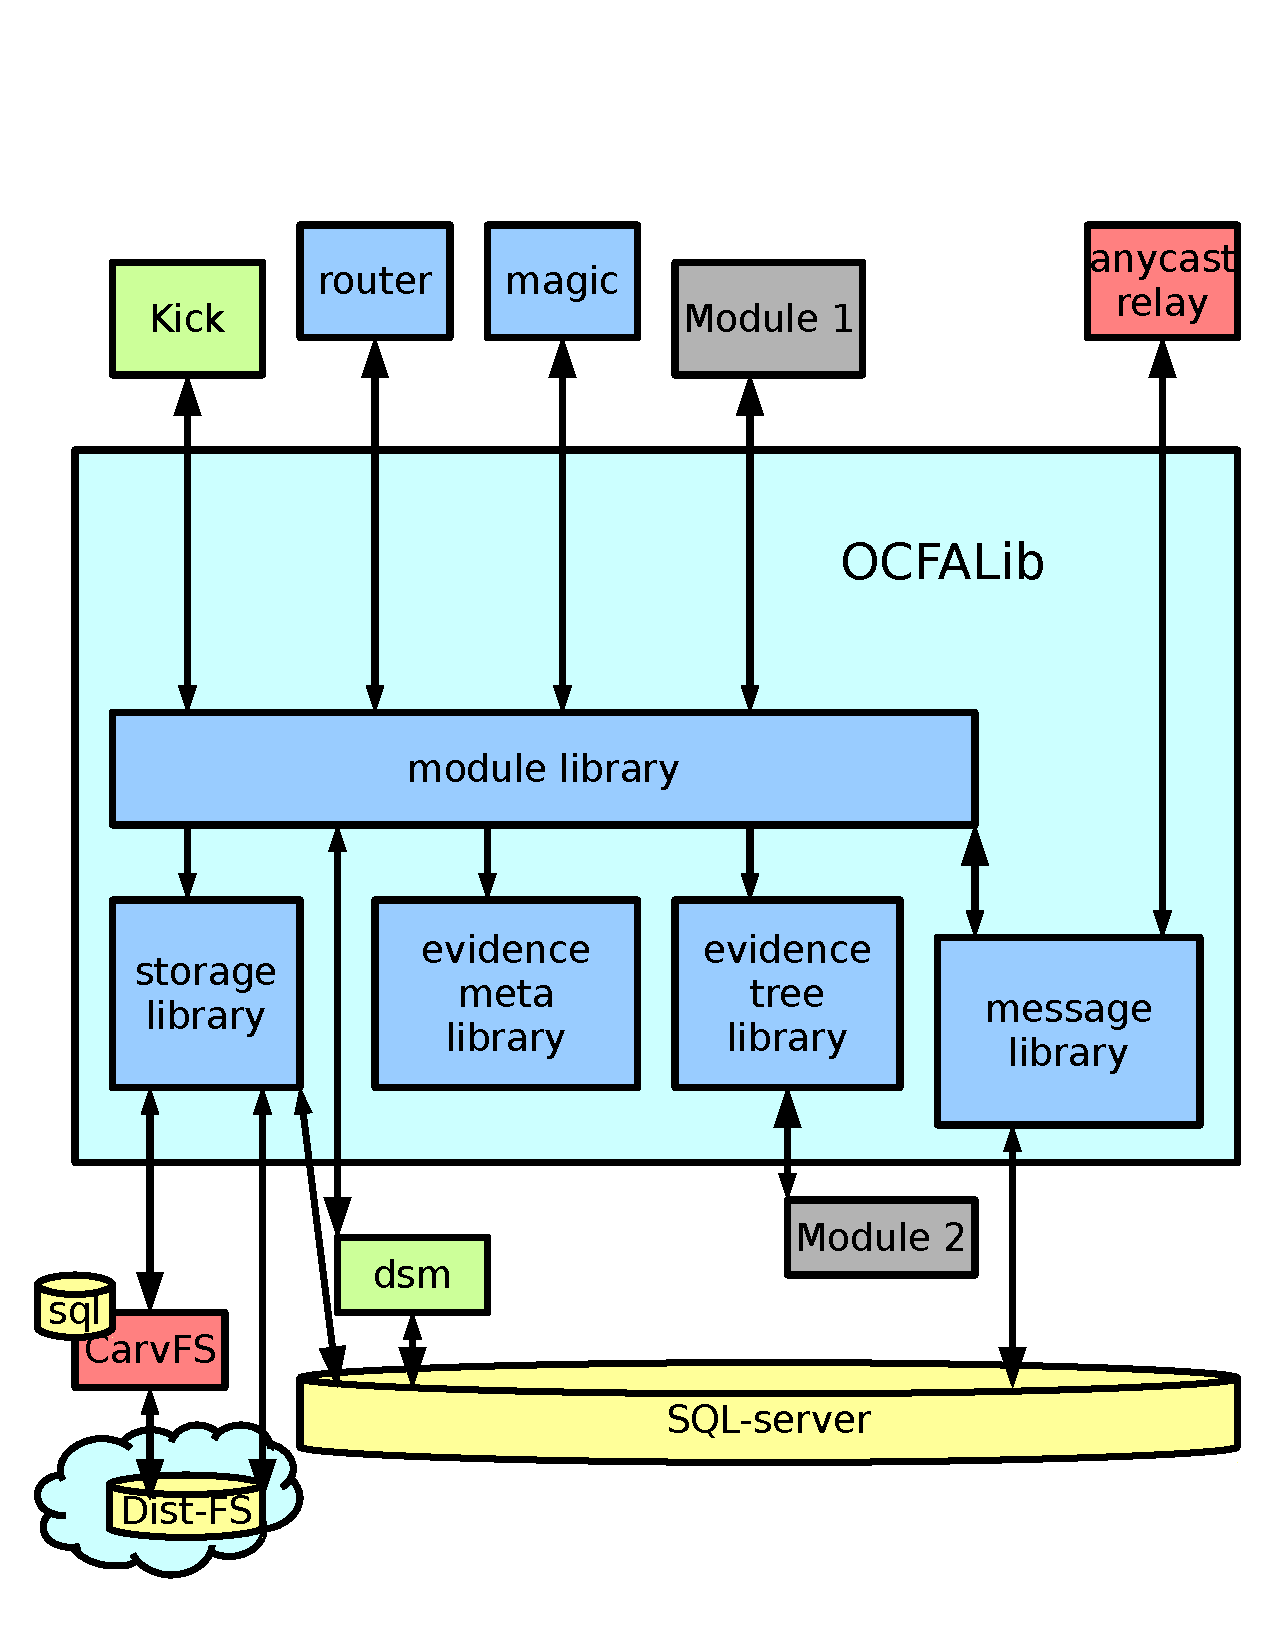
\includegraphics[width=100mm]{mattock/libraryview.pdf}
\caption{The base OCFA architecture}
\label{fig:FlowInOut}
\end{figure}
If we look at the OCFA architecture, at the core we basically see a fully custom build asynchronous messaging framework for processing modules that communicate with a small set of networking components that act to combine the modules into dynamic chains of tools that are applied to parts of the forensic evidence data. The use of commodity software components is mostly limited to the pervasive use of XML technology and a central relational database. We shall have a look at some of the core components of the OCFA framework.
\subsection{The AnyCast Relay and Persistent Priority Queue}
At its basis, OCFA was a message passing concurrency based system. One known issue with message passing concurrency is the use of buffers. While message passing environment like the Erlang programming language and platform opt to put producing processes to sleep when buffers fill up, OCFA opted for a different approach. In OCFA, the message passing buffers were managed by on-disk persistent priority queues. These queues only contained referenced to in database large text objects. The persistent queues were meant and designed to be fully crash resistant. The priority queues had a special \emph{'never'} priority to hold messages that were observed to crash specific modules. This allowed modules to be restarted and to skip problematic data until a maintenance programmer would look at the problematic data and buggy module to fix the problem and re-submit the messages in the never queue for further processing. The AnyCast relay was built on top of the persistent priority queue. Every module connected to the AnyCast relay and registered as a consumer of a certain type (a module \emph{instance}) and would go into a message processing event loop asking the AnyCast relay for new jobs. When a module was done with a piece of evidence data, or when a module derived a sub entity from such data (for example an attachment as child entity of an e-mail message), the module would send a message to the AnyCast Relay addressed at a special process named the \emph{router}. The AnyCast would keep track of irresponsive and broken network connections and would play an important role in having stale or crashed modules restarted in a way not unlike what is common practice in Erlang based architectures. On such a detected crash, messages that were still pending a response would be put aside in the never queue to be looked at by a technician at a later point in time. In OCFA the AnyCast relay served as a single server for all modules, independent of the server these modules would run on.
\subsection{OcfaLib, a domain specific asynchronous framework}
While today NodeJS has mainstreamed the idea of a generic asynchronous framework, and while in other programming languages generic asynchronous frameworks such as Twisted for Python or Boost::asio for C++ have been available for quite a while, OCFA was first built long before such systems became mainstream. As a result, OCFA basically ended up building its own asynchronous processing framework. We could say that OcfaLib, the C++ OCFA library was a domain specific asynchronous framework for use with the AnyCast server. 
\subsection{The legacy Module API}
OCFA came with two quite distinct module Application Programming Interfaces (APIs). This fact was the result of chronology of development. The first version of OCFA came with a module API not much unlike that of the current day Sleuthkit framework. A module would get a file to process and could add meta data to that file, or, when it wanted to for example mark an extracted e-mail attachment as child entity, would submit that to the framework. The API consisted of a module initialization part and a single method called 'processEvidence' that a module was supposed to overload. From within processEvidence the module could either add meta or submit a child entity with added meta date.
\subsection{The Tree-graph API}
After new modules got added to OCFA, the legacy module API was found to be lacking in the meta-data area. The problem was that a module deriving a tree of children would not be able to set meta-data for deeper child entities. Only level zero and level one meta data was possible. As a result, the more powerful tree-graph API was added. As porting old modules to the new API was considered a waste of precious development time, the old API was also still continued after the introduction of the new API.
\subsection{The legacy CAS storage}
OCFA in its initial release came with a Content Address Storage system for storing data entities. Data was created or, lacking CarvPath facilities, first copied to a temporary file and hashed during copy. Once the hash was fully calculated, the temporary file was either moved to a location derived directly from the hash of its content, or discarded if an entity with the same hash was already present in the repository. 
\subsection{CarvFS}
Later releases of OCFA were made compatible with the use of CarvFS for parts of the storage needs. CarvFS integration has however remained a bit of a hack. The storage sub-system of OCFA used physical symbolic links to CarvFS CarvPaths inside of its primarily CAS based storage system. This meant that for example when using a CarvPath aware Sleuthkit MMLS module, storage of a partition in the OCFA CAS storage system required the full partition to be read for hashing purposes before it could be symlinked in the storage subsystem.
\subsection{The meta-data based message router}
At the core of the OCFA architecture was the central meta-data based router. This XML technology based router would parse the meta-data that modules had gathered on a data entity and would based on an also XML-based rule-list determine the next hop in the tool-chain for that data entity. 
\subsection{The use of an SQL server}
There were two technologies that were pervasively used within OCFA. One XML we already discussed. The second one was a relational database. It was used by the storage subsystem, by the messaging subsystem, and finally by the meta-data storing data-store-module. In each of these uses, the use of an SQL database turned out to be a sub-optimal choice for a number of reasons. Some related to the creation of run-time performance bottlenecks and others related to the nature of the data structure and the nature of useful analysis-time queries on this data. More on this when we discuss the alternatives for Mattock.
\section{PyFlag}
\begin{figure}
\centering
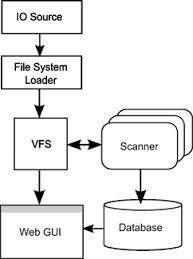
\includegraphics[width=50mm]{mattock/pyflag.jpg}
\caption{The base PyFlag architecture}
\label{fig:FlowInOut}
\end{figure}
Next to OCFA, the PyFlag framework deserves mention in this paper. While PyFlag has quite a different scope than OCFA it shares a lot of similarities too. Where OCFA is meant purely as a framework for computer forensics, PyFlag is a hybrid system that also addresses the field of network forensics. This hybrid approach makes that this framework would in a fundamental way be much more difficult to apply disk-cache related optimizations. It thus would be unfair to look at PyFlag purely from a large scale computer forensic data processing point of view in a comparative way. 
\section{The Sleuthkit Hadoop framework}
A more promising development was the Sleuthkit Hadoop framework. It aimed to combine The Sleuthkit with specific distributed technology. The technology proposed was a combination of the HDFS distributed file-system and the distributed NoSQL database HBASE, both part of the Hadoop technology stack. These two technology choices are absolutely take-away points we need to copy when implementing Mattock. That is, a distributed file-system and NoSQL technology. We shall look in more detail at suitable NoSQL technology. While HBASE isn't a bad choice at the processing end, there are data structure and analysis concerns that would point to different NoSQL technology as potentially more suitable. 
\section{Non-open frameworks}
It is important to note that due to the closed nature of the frameworks involved, this paper does not look into some major and widely successful non-open forensic frameworks such as Xiraf or FTK Distributed Install. The scope of this appendix is limited to open tools and publications.
\section{Digital Evidence Bags}
So far we have been looking purely at scalability and performance of forensic architectures without considering other important new computer forensic insights. One conceptual idea that all current frameworks seem to discard are the key concept introduced with so called Sealed Digital Evidence Bags (SDABs) by Bradley Schatz and Andrew Clark in 2006. While the details of SDABs fall outside of the scope of this appendix, one key aspect deserves special attention: The concept that both data and meta-data require a form of tamper-proofness. That is, once a piece of evidence data or meta-data is entered into the system, this (meta-)data should be considered to be logically immutable. We shall take this concept with us in our outlines for e next generation scalable framework.
\section{New insights}
Looking back at OCFA and other forensic frameworks, there are in retrospect important suboptimal choices that would be made differently if a framework like that was to be developed today. In this section we summarize a few important insights that arose from years long usage of OCFA, a survey of other open frameworks. A literature survey and the results of the timing analysis in the first appendix of this paper.
\begin{itemize}
\item \emph{A tree-graph API is essential} : While simpler API's can be useful for some trivial modules, all such modules could also work with a more generic tree graph API. Having just one generic tree-graph oriented API could facilitate a much wider range of modules and if the API is defined in asynchronous terms, the API could be portable to alternative architectures.
\item \emph{Leveraging asynchronous frameworks is essential} : OCFA implemented its own custom asynchronous framework and the part of the OCFA code-base involved with implementing that functionality was substantial. With current day asynchronous frameworks such as Boost::asio (C++), Twisted (Python) or NodeJS (JavaScript), the need for a custom built asynchronous framework has disappeared.
\item \emph{Evidence sealing facilities are a must} : It is essential to limit the mutability time-span and scope to an absolute minimum. Both from an anti-forensics point of view, and from the point of view of the legal credibility of the integrity of the implemented forensic process.
\item \emph{Reducing disk-cache misses is essential for performance}: While many papers focus on CPU cycles being wasted by inefficient forensic processes, the truth is that much of the forensic process is IO rather than CPU constrained. As such, the fact that the same data \emph{will} get read multiple times should make clear that a disk-cache miss will impact throughput and that a forensic framework such as OCFA with a design that does not effectively mitigate disk-cache miss rates will suffer from throughput disk-cache-miss related IO bottlenecks.
\item \emph{Zero-storage carving is essential} : The process of locating, carving and validating files on disk images is complex and will either result in high false positive or high false negative counts. In the case of high false-positives, copy-out will result in massive needs for forensic archiving storage for derived entities. In the case of high false negatives essential data may be missed. Applying zero-storage carving facilities such as CarvFS will allow for a relatively low cost of false positives while minimizing the amount of additional storage required for processing.
\item \emph{Simple priorities don't really work} : While our research has shown that priority queuing as used in OCFA would be effective for homogeneously sized chunks of evidence data, not taking into account the size of the evidence entities and their likely disk-cache status in prioritizing has been shown to yield such poor results that the usefulness of priority queuing in such a way must be seriously questioned. 
\item \emph{Current day forensic disk image formats are poorly suited for large-scale processing archives} : In large scale investigations encompassing dozens to hundreds of full-size disk images, the in-lab usage of the common computer forensic disk image storage formats (EFF \& AFF) have shown to be rather poorly suited. Lacking a forensic lab storage format for large archives of disk images, the use of simple sparse dd images or basic directory tree with copied out files as underlying lab storage format seem to both be vastly better than. It would be ideal if future research would investigate the possibilities of archive friendly storage of computer forensic data.
\item \emph{Data migration should not be taken lightly} : While distributed file-systems or storage systems such as SNFS can facilitate in making evidence data available on many nodes, it is important to realize that accessing data from a different node will per definition result in a disk-cache miss on that node. It is suggested that data migration should prefer either the early out-of-cache migration of data that has not yet been fully cached by the originating module, or the migration of relatively small chunks of data targeted for relatively high-CPU processing on the other node. 
\item \emph{Relational (SQL) databases are a poor fit on all fronts} : In OCFA the Postgress SQL database was used for many things. In retrospect, certainly given the current day alternatives, these things would today all have better alternatives. First of all, the database usage for \emph{mutable} meta-data and for the storage and messaging subsystem together was a major performance bottleneck. Apart from the fact that in retrospect in-process mutable meta-data does not fit in with the SDEB view of things, a relational database is a poor choice of technology for implementing either such meta-data \emph{document} storage or the extra indirections implemented within the storage and messaging subsystems. More than that though, the usage of an SQL database by the data storage module and the user interface have shown that many of the more advanced analysis's have had such shape and form that the database and queries would have been much better of having a more \emph{graph} oriented infrastructure. If we look at OCFA and than look at modern NoSQL technology, we see that parts of the SQL functionality had better be implemented without a database, some had better be implemented with a distributed \emph{key/value store} database, some with a \emph{document} database and some with a \emph{graph} database.  One thing all aspects of OCFA have in common is that SQL technology in todays technology landscape would be a sub-optimal choice at best. 
\item \emph{Kick-starting may not start at a server node} : In OCFA kick-starting took place from a server node. Before this could be done however, the EWF files had to be placed on an SNFS partition accessible to the server from a client through an SNFS connected file-server. Combine this with the need for converting EWF to dd or an other lab friendly format, the lack of a client-based EWF submitter led to massive disk write inefficiency. A kick-starting network client would need to be an essential component in a modern forensic framework.
\item \emph{Not all modules are alike} : All open forensic frameworks treat modules as equal citizens. The reality however is that some modules such as a file-type module are so common in data processing that framework embedding would be justified, some modules such as simple carvers are used mostly on huge data files and are IO intensive while others like OCR work on relatively small data chunks and take up significant CPU resources. Treating all modules and all data as similar will inevitably lead to poor overall framework performance. 
\item \emph{Globally valid annotations are the key} : As each server in a forensic data processing cluster has its own disk cache, the concept of dividing the load between different nodes by distributing and redistributing to different nodes should be positively influenceable by allowing nodes to have a common communicable notion of the portions of the global investigation data they and other nodes likely still have in their cache. For this, a globally valid annotation for data chunks is essential CarvPath annotations could play a major role in this.
\item \emph{Meta-data serialization technology matters} : At the time that OCFA was devised, XML was the only logical choice for meta-data serialization. The XML technology stack though is far from being the most efficient serialization form for forensic meta data. While there are multiple papers proposing standardized XML formats for forensic meta-data exchange, the inefficiency of XML forms a major bottleneck in event-rich high throughput processing such as in a computer forensic framework. More efficient serialization options such as JSON, Protocol Buffers or Cap'n Proto should be seriously considered as alternative to XML. 
\item \emph{Hashing algorithm choice is essential} :  Traditionally MD5 and later also SHA1 have been used as hashing algorithms in digital forensics. From a cryptographic point of view, MD5 is now deprecated while SHA1 is in the process of being deprecated. Many public and law-enforcement-only hash collections like the Virusshare hash set or national child pornography hash sets are still distributed only with MD5 and/or SHA1 hashes. Others like the NIST NSRL are now supplemented with SHA256 hashes. While the later may sound like good news, there is an other important issue with SHA256 for use in a forensic framework: SHA256 may be significantly more secure as a hashing algorithm than SHA1 or MD5, it is also significantly more CPU intensive. So much so that it may undermine the whole concept of opportunistic hashing as presented in this paper. While today NIST still considers the use of SHA1 for purposes as defined in this paper as \emph{acceptable use}, we must consider the retroactive impact that a cryptographer testifying on behalf of the defense and questioning the use of SHA1 in the forensic process may have a few years from now if SHA1 reaches the same level of deprecation that MD5 has today. It thus can be argued that moving forward to a non-deprecated secure hashing algorithm should be considered a priority. Given the CPU resource issues with SHA256, it is also of paramount significance that the algorithm we move forwards to should have at least reasonable resource requirements in its software implementation. A quick study into available secure hashing algorithms reveals a small family of secure hashing algorithms. SKEIN, BLAKE and BLAKE2 share properties that would make each of these secure hashing algorithms prime candidates for supplementing and eventually replacing SHA1 as primary hashing algorithm for computer forensics. In the next appendix we will make the case for one of these. The important insight here however is the notion that SHA1 is close to deprecation, SHA256 puts to much strains on resources in a high performance computer forensics setup and we need to pick a more suitable replacement.     
\end{itemize}
\section{A modernized OCFA inspired open-source architecture}
With the good parts from the old OCFA architecture combined with the new insights above, we can sketch the base outlines of a next generation message passing concurrency open computer forensic framework. Let us start out with a rough description of the changes from the OCFA architecture to our new Mattock architecture outline. We see that the custom asynchronous framework gets replaced with boost::asio and twisted for the respective C++ and Python languages and that Python replaces Java as secondary platform language. We see that file-type logic and meta-data router are no longer a separate module and network service but are now integrated in the base functionality for each module process. Further we see the number of module APIs reduced to just the tree-graph API. The most obviously notable change however is the fact that there is no longer a direct dependency between generic modules and database technology. The SQL server has disappeared and has been replaced by other technology. The Data Store Module (DSM) maps the meta-data into a NoSQL database. This will most likely be a distributed graph-database or a distributed document-database (or possibly a hybrid combination of the two such as ArangoDb. Both data and now also meta-data are stored in a write-once way to the CarvFS replacement MattockFS that implements a subset of the SDEB concept by means of privilege separation and immutability. The CarvFS long-path SQL database is replaced with a distributed key/value NoSQL database. While MattockFS should initially still run on SNFS or NFS, the use of a distributed file-system such as HDFS should be a potential way forward to further improve scalability. The AnyCast Relay is replaced by a similar AnyCast monitor mesh-up. One node per worker host. A AnyCast monitor will be a redesign of the AnyCast that is fully CarvPath aware and is able to monitor a full worker host, both through the proc filesystem and through communication with MattockFS. The kick-starting process is revised. EWF processing is moved to the client side of things. The client connects to a central kick balancer that will query all AnyCast monitors to find the right kick server to redirect the client to. 
\begin{figure}
\centering
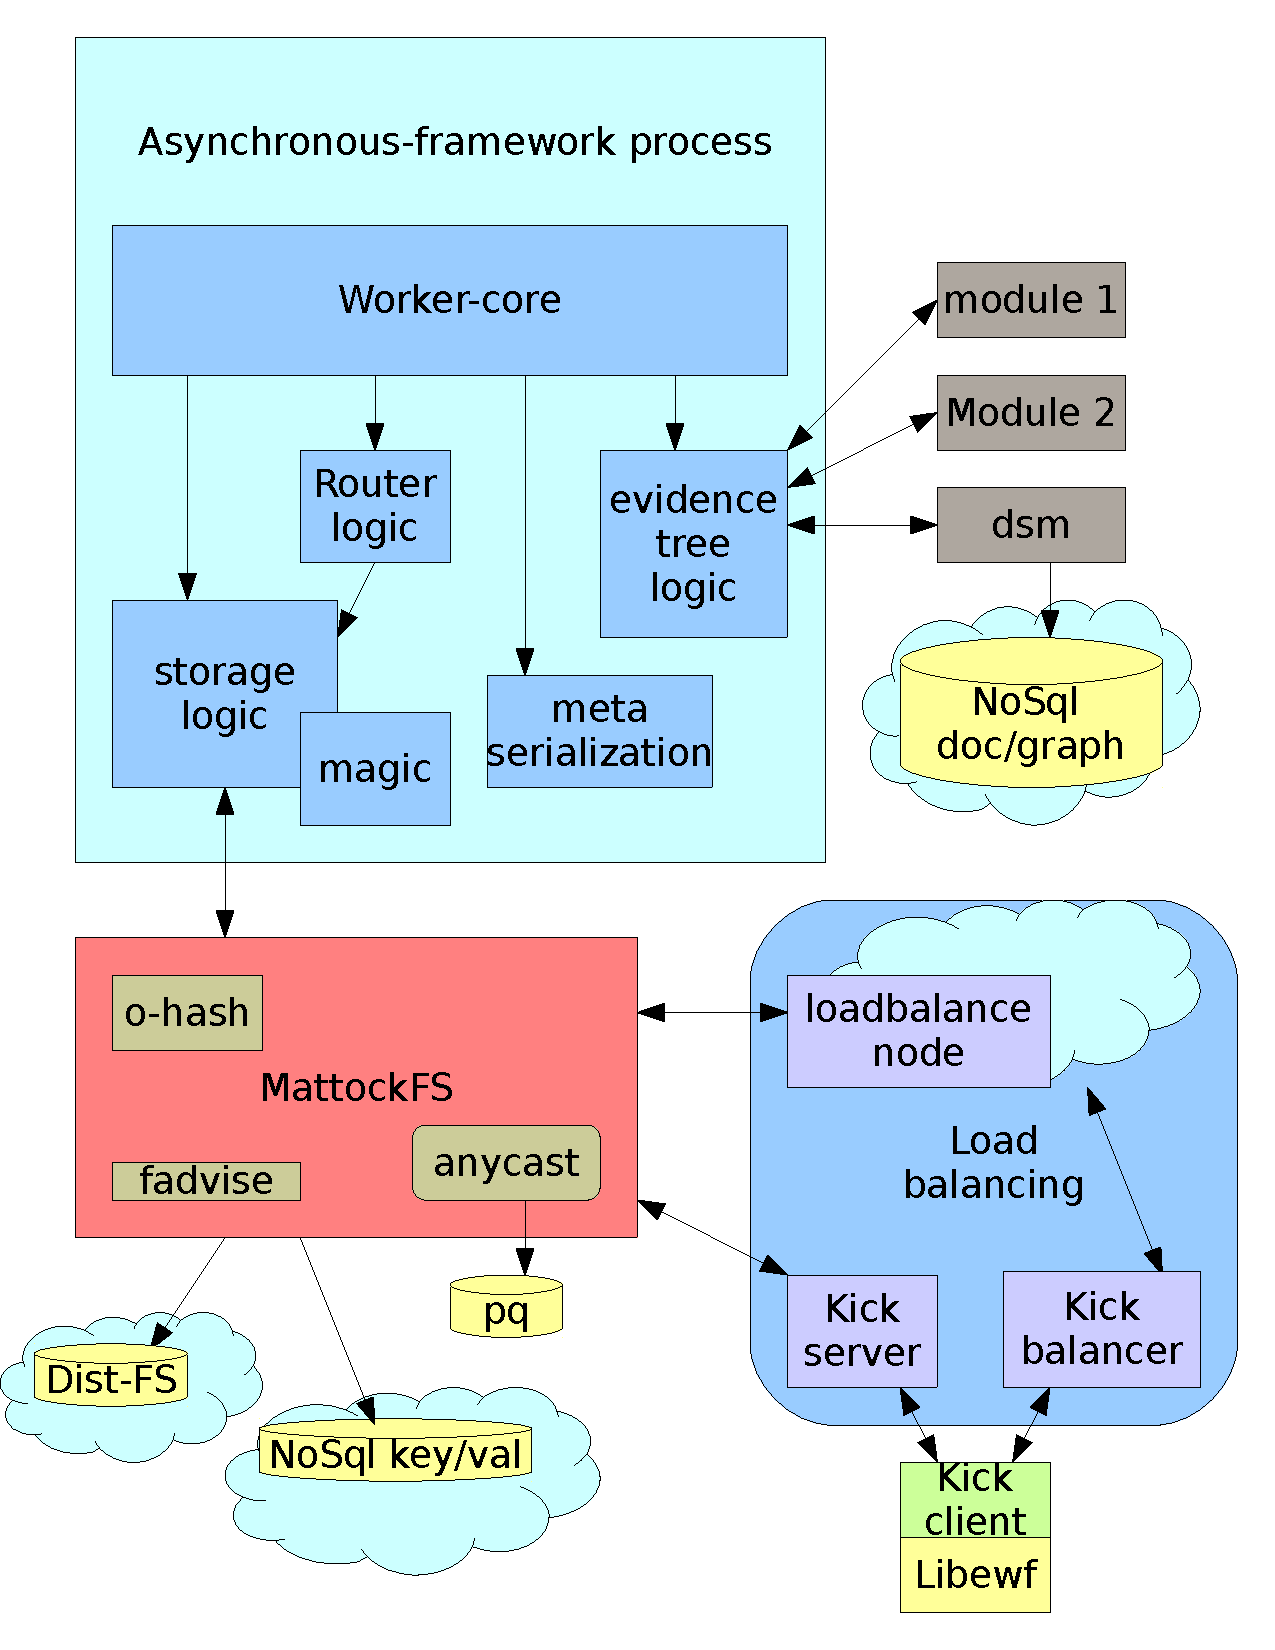
\includegraphics[width=100mm]{mattock/libraryviewmattock.pdf}
\caption{The base Mattock architecture}
\label{fig:FlowInOut}
\end{figure}
\subsection{The distributed long-path store}
\subsection{SNFS vs HFS}
\subsection{MattockFS \& the distributed long-path store}
\subsection{Effective distributed system usage}
\subsection{The AnyCast Monitor mesh-up}
\subsection{Client/Server kick-starting}
\subsection{Store-system embedded lib-magic functionality}
\subsection{Distributed routing logic}
\subsection{From SQL to Graph based NoSQL}
\subsection{Using language-native asynchronous frameworks}
\subsection{A single tree-graph, lambda and asynchronous operation oriented API}
\subsection{Conclusion}

\include{mattock/other}
\chapter{MattockFS}
In this appendix we describe the functionality and design of a new user-space file-system. MattockFS is meant to be a successor to the user space file-system named CarvFS that was released by the Dutch National Police to act as an annotation based pseudo file-system aimed at facilitating zero-storage carving to the OCFA forensic framework. While CarvFS was retrofitted to work with OCFA, with MattockFS we aim to create a new user-space file-system modeled partially after CarvFS that should act as the potential foundation of new message passing oriented forensic framework. We envision that MattockFS, together with a shared key/value store,a serialization library and OCFA-Anycast like message bus technology could form the foundation for an envisioned future \emph{Mattock} forensic framework. The aim is to implement as much as is logical and sensible of the main aspects of disk-cache optimization techniques into this user space file-system. This should include facilities for querying throttling relevant information, facilities for keeping track of \emph{active} CarvPaths, facilities for marking expected read-access patterns for a given CarvPath and for marking a CarvPath as no longer needed. Also it shall include facilities for opportunistic hashing. Finally, while in OCFA, the concept of a growing archive was implemented by allowing a data-generating module access to the raw data-file underlying the file-system, in MattockFS we shall opt to implement this trough a file-system layer. This file-system should have the potential of becoming one of the foundational stones for the construction of a next generation open source message-passing concurrency based computer forensics framework. We shall refer to this envisioned framework that will need to interact closely with MattockFS as the Mattock framework or i\emph{Mattock} for short.
\section{FUSE: File-system in user-space}
In Linux, a file-system will normally reside in kernel-space. Sometimes statically as part of the main kernel, and often as a kernel loadable module. While from a performance point of view, kernel-space file-systems are preferable, writing software to run in kernel space is quite challenging and comes with many pitfalls. Most software libraries that are available in user-space are unavailable in kernel-space, and even much of the standard OS API functionality is not accessible in the same familiar and convenient access patterns. next to these concerns, there are security implications to the concept of running a large body of programming logic at the level of a trusted kernel module. As an alternative to kernel level file-systems, the Linux kernel comes with a special file-system loadable module and an accompanying user-space library that together are aptly named FUSE. FUSE is an almost-acronym that stands for Filesystem in User-space. The kernel module communicates with the library and together they allow the creation of a regular user-space process that performs the task of being a file-system. MattockFS, like CarvFS before it, aims to be such a user-space file-system. 
\section{MattockFS functionality}
MattockFS aims to become a successor to CarvFS, implementing the facilities needed for doing zero-storage (also  named "in place") file carving within the context of a computer forensic framework as CarvFS did, but also implementing a range of functionalities that aid in reducing the page-cache-miss-rate for the Mattock framework that it facilitates. Next to this, MattockFS shall implement some facilities relating to mutable data access that should contribute to the overall robustness of the framework and the integrity of the forensic process.
\subsection{The concept of concurrent pseudo-batches}
While processing of data in a forensic frameworks is something quite dynamic, when seen from MattockFS we can look at it as a large number of concurrent pseudo-batches. Each batch works on one specific piece of data as designated by one specific CarvPath. A batch consists of a set of operations on the data, each operation done by one specific framework module. A set of operations that has a beginning and an end. As such, from the point of view of the file-system, the framework and the file-system cooperate in completing pseudo-batches that are designated with the same CarvPath that also designates the data that the batch works upon. This concept of pseudo-batches is an important concept in each of the sub-responsibilities of MattockFS.
\subsection{Adding data to the archives}
In OCFA the concept of a \emph{growing archive} was introduced. The idea of a growing archive is that a large raw data file is made available through a filesystem like CarvFS of MattockFS, and that data entry processes (called kickstarts in OCFA) and data derivation processes (called dissectors in OCFA) are allowed to \emph{grow} the underlying raw data file that the file-system runs on top of. One major drawback of this approach was that the growing archive would need to be writable to each and every data producing kickstart or dissector (or as in OCFA, each and every module). Each module, or tool invoked by a module, then has the power not only to add new data to the archive, but also to potentially corrupt the existing archive. Given the reality of both anti-forensics and of software bugs in many data processing tools that might be used from within the context of a forensic framework, this approach is undesirable from a robustness and data integrity point of view. To alleviate this concern, MattockFS will implement an add-only interface for allowing Mattock modules to enter or derive data without being able to modify any of the data that was entered into the filesystem at an earlier point. Not only for data that was entered by other modules but even to the extend of not allowing mutable state to exist in any data that was fully submitted by the same module itself. MattockFS shall ensure both exclusivity of access during creation and immutability of data after it has first been fully submitted by its creator.
\subsection{Annotation based data access}
As in CarvFS, the core of the functionality of MattockFS is centered around the concept of annotation based access to data. CarvFS defined a convention for annotations named CarvPath that MattockFS will be adopting. This convention can be summarized as:
\begin{itemize}
\item CarvPath annotations can be nested like directories separated by a directory separation character as defined for the particular OS. For Linux that character is '/'. In a multi layered CarvPath, each level designates a CarvPath relative to the directory level above it. MattockFS (like CarvFS before it) will \emph{flatten} all multi-level CarvPath annotations by representing second level CarvPath entities as symbolic links to their first level \emph{flattened} representation.
\item Each CarvPath annotation comes in two forms. The \emph{directory} form that consists of just the CarvPath without a file extension, and the \emph{raw} form that is denoted using the same CarvPath, but postfixed with the \emph{.crv} file name extension.
\item A CarvPath can denote a fragmented entity within its parent. In such a case, the character '\_' is used as a separator between the fragments.
\item A \emph{normal} fragment consists of two decimal numbers separated by a \emph{'+'} sign. The first represents the offset within the parent entity. The second number denotes the size of the fragment.
\item A fragment can be defined as being \emph{sparse}. This means there is no actual data there, and if the data is read, all zeroes will be returned. A \emph{sparse} fragment is denoted as a capital \emph{'S'} followed by the size of the sparse fragment in decimal form.
\item A CarvPath may end up being longer than the OS file-system allows a directory level to be. For that reason a CarvPath annotation for a really long very fragmented CarvPath may be replaced with a digest of the CarvPath. Such a digest/CarvPath mapping will need to be stored in order to allow usage of the digest for accessing the underlying data. Note that this aspect of CarvPath annotations creates a challenge for distributed usage of CarvPath annotations. We shall discuss these concerns further down below.  
\end{itemize}
\subsection{Framework usage vs interactive usage}
The initial version of MattockFS prioritizes usage from within a framework context over interactive usage. As such performance in the interactive usage of MattockFS could be sub-optimal. It is recognized that in a real operational environment the interactive usage and framework usage will often occur simultaneous and may thus intervene with each-other. This is left as a subject for further study that falls outside of the context of this research project. We shall act as if interactive usage of MattockFS will be rare. We shall focus on MattockFS usage from within the context of pseudo-batches. Optimization of non-pseudo-batch usage is considered as an important subject, yet a subject that is not within scope for this research project.
\subsection{Page usage control, monitoring \& release}
MattockFS, when looking at it from a distance, is nothing more than a fancy wrapper for an open file handle to a huge (growing) raw archive-file. MattockFS will try to, using the \emph{fadvice} API as described in the previous appendix, in order to communicate with the kernel about keeping or no longer keeping pieces of the huge raw archive-file in the page-cache. So when should MattockFS mark a certain section of our archive to be kept or released from the page-cache? Its a quite delicate process involving reference counting, pseudo-batch marking and the opening and closing of pseudo files within the file-system. A brief outline of a simple strategy:
\begin{itemize}
\item When a batch is marked, all space indicated by the batch has a \emph{WILLNEED} reference counter incremented.
\item When a batch is unmarked, all space indicated by the batch has a \emph{WILLNEED} reference counter decremented.
\item When a pseudo file is opened, all space indicated by the pseudo file  has a \emph{NORMAL}  reference count incremented.
\item When a pseudo file is closed, all space indicated by the pseudo file has a \emph{NORMAL} reference count decremented.
\item Whenever needed, fadvice is invoked for an area resulting from reference counter values. The last \emph{advice} for any given region needs to be;
\begin{itemize}
\item \(WILLNEED == 0 ; NORMAL == 0 \Rightarrow FADV\_DONTNEED \)
\item \(WILLNEED == 0 ; NORMAL > 0 \Rightarrow FADV\_NORMAL \)
\item \(WILLNEED > 0 \Rightarrow FADV\_DONTNEED \)
\end{itemize} 
\end{itemize}
MattockFS will be keeping track of these reference counters, and as such will be able to keep track of what it has asked the kernel to keep in page cache. This information will proof useful for our throttling control later on.
\subsection{Throttling control}
While MattockFS itself does not concern itself with throttling, it is in a unique position to provide data providers within the Mattock framework with information that should proof useful then implementing effective throttling strategies. The throttling related bookkeeping in MattockFS consists of three distinct parts:
\begin{itemize}
\item The file-system provides information on the total amount of file fragment that are marked as FADV\_DONTNEED or FADV\_NORMAL.
\item As MattockFS handles read operations, and as the kernel provides the \emph{mincore} API call for checking if a page to be read resides in the page cache, MattockFS provides information as to the recent success rates with regards to page cache hits.
\item A data producing module may issue a \emph{what if} query regarding a CarvPath. This query will return the expected growth in page-cache demand resulting from consecutive marking of the CarvPath as a pseudo-batch.
\end{itemize}
The combination of these three sources of information from MattockFS should allow the modules in the framework to delay marking new pseudo-batches until old pseudo-batches have completed, possibly by throttling using the messaging subsystem.
\subsection{Opportunistic hashing}
Next to the whole \emph{fadvice} and throttling part, the concept of pseudo-batches also comes into play when implementing our opportunistic hashing. Whenever the combination of the two reference counters goes from zero to one, an opportunistic hashing context is initiated and an offset is initiated at zero. Now whenever, during the lifetime of the batch, a piece of data is read that roughly connects to the offset location, than an opportunistic hashing operation that hashes part of the data and forwards the hashing offset is attempted. If the connection isn't seamless but close, \emph{mincore} is used to check if the intermediate space happens to already be in page cache. Further, the pages directly following the requested data are also checked using the \emph{mincore} operation. Whatever chunk of in-core data can move the hashing offset forward will be used to do so.
\subsection{Choice of algorithm}
If we discard the interesting and important efforts in the fields of partial and fuzzy hashing and focus on full-entity hashing, there are four main ways how hashes are used in computer forensic processing.
\begin{itemize}
\item Check against known good. This includes abandoning further processing for for example Windows OS system files.
\item Check against known bad. This includes marking for example known child pornography image files.
\item Check against \emph{seen before}. This can keep a forensic framework from for example unzipping a large archive that is found in many places for every place where it was found.
\item Applying set-theory to groups of files from different sources within a single investigation. This includes things like allowing an investigator to select all office documents unique to the intersection of office files found on the systems of two suspects.
\end{itemize} 
For the first two purposes, compatibility of the hashing algorithms used in the known file hashes data set with the hashing algorithm used by the framework is important. For the other two purposes there exists only one algorithm; the one used by the framework. It is with the first two types of usage that we run into an issue witch choosing a hashing algorithm for MattockFS. The problem is that data-set producers seem to be behind the curve with regards to secure hashing. Many known-file data-set providers only provide SHA1 hashes. According to NIST, SHA1 is deprecated for the \emph{generation} of secure hashes (as was MD5 before it). Even NIST though still distributes their \emph{NSRL} known-file hash data-set with (next to SHA256 hashes) SHA1 hashes.  The apparent reason for this is that the secure SHA256 hash has very poor performance when used in software. As use of hashes in computer forensics involves the hashing of large amounts of data, and as access speeds to that data are increasing as the use of solid state disks in CF setups gains more traction, the poor performance of the more secure SHA256 becomes a serious performance consideration. There are several alternative hashing algorithms that combine a strong and secure hash with a decent or good performance on a software platform. Most notably two (non-winning) candidates for SHA-3: SKEIN and BLAKE. Those however come with a lack of compatibility with our dataset providers. Finally, a successor to BLAKE, BLAKE2bp comes in forms optimized to take advantage of 64 bit multi core systems. We must acknowledge though that SKEIN and the original BLAKE, as being part of the SHA-3 competition will likely have been more scrutinized than BLAKE2, so our trust may be slightly less in that algorithm. A short overview :
\begin{table}[]
\centering
\begin{tabular}{llllr}
Algorithm & Secure & Trusted & Compatible & Speed compared to SHA1 \\ \hline
SHA1 & NO & YES & YES & 100\% \\
SHA256 & YES & YES & YES & 30\% \\
SKEIN & YES & YES & NO & 75\% \\
BLAKE2b & YES & NO* & NO & 135\% \\
BLAKE2bp & YES & NO* & NO & 420\% \\
\end{tabular}
\end{table}
When we look at the numbers above, we can conclude that combining SHA1 with the multi-core 64 bit optimized BLAKE2bp algorithm will give us at least the security of SHA256 combined with the compatibility of SHA1 at a performance hit of only 20\% when compared to only using SHA1. We pose that a final version of MattockFS shall support the following modes and algorithms for the user to choose between:
\begin{itemize}
\item SHA1 only (100\% speed; compatible/insecure)
\item BLAKE2bp only (420\% speed; incompatible/secure)
\item Dual hashing (80\% speed; compatible/secure)
\end{itemize} 
Within the context of the initial version of MattockFS that falls within the scope of this research project, we shall implement only one of these modes.
\subsection{Distributed access concerns}
Given that MattockFS at its basis is an overlay file-system, much of the distributed access can be addressed by storing the raw archive file on an underlying file-system with distributed access. This could be something like a StorNext File System (SNFS) that allows multiple servers fiber channel access to the same data, or something like a simple NFS share. This part falls outside of the scope of concern for MattockFS.
There is however one essential distribution concern not directly related to distributed file-systems: The digest representation of long CarvPath annotations. We shall make sure that MattockFS allows for a loosely coupled link to a key/value store system that is usable in a distributed setting. A system such as \emph{Redis} would appear like a good match for such functionality. 
\section{Basic directory structure}
MattockFS uses the following base directory structure:
\begin{itemize}
\item \emph{data.crv} : A pseudo file representing the entire archive.
\item \emph{data/} : The top level for CarvPath access to the data.
\item \emph{mattockfs.info} : Empty pseudo file for file-system level interaction.
\item \emph{newdata/} : Pseudo directory for entering new data.
\end{itemize}
The data.crv file and data/ directory work in exactly the same way that CarvFS did. Nested CarvPath annotations redirect to first level flattened CarvPath annotations that are than accessible as pseudo files. What is different about the data directory is that the pseudo files inside of it allow for a close interaction of the framework using MattockFS with the throttling, page-cache management and opportunistic hashing logic inside of MattockFS and indirectly with the page-cache control functionality within the Linux Kernel. This interaction is done through the use of an extended attribute based control mechanism. Some interactions don't make sense on a per-CarvPath basis and are done against the MattockFS file-system as a whole. For that reason the pseudo file mattockfs.info acts as a front for MattockFS as a whole. This file comes with its own distinct extended attributes. Finally the directory newdata. This directory allow each distinct process accessing MattockFS to create a new pseudo file what's content is to be appended to the growing archive underlying the file-system. 
\section{CarvPath level attribute based control and info}
At the level of individual CarvPath annotations, extended attributes are to be used to interact with MattockFS. We define the following attributes:
\begin{itemize}
\item \emph{batch} : Settable boolean variable denoting if framework or script will access this CarvPath again with an other module soon. If \emph{true} MattockFS will attempt to have the kernel keep the accessed part of this CarvPath in the page-cache until set to \emph{false}. Setting \emph{batch} to \emph{true} will also initiate opportunistic hashing for the CarvPath.
\item \emph{advise}: Read only value denoting the currently set \emph{advice} value as set for the CarvPath.
\begin{itemize}
\item \emph{normal}: Set to POSIX\_FADV\_NORMAL
\item \emph{willneed}: Set to  POSIX\_FADV\_WILLNEED
\item \emph{dontneed}: Nothing set or explicitly set to POSIX\_FADV\_DONTNEED.
\item \emph{ambiguous}: Different parts of this CarvPath have a different status.
\end{itemize} 
\item \emph{incore} This attribute represents two distinct operations. When read, this variable will return a boolean indicating if the CarvPath is available in full from the page-cache. When set to \emph{true}, the CarvPath is set to POSIX\_FADV\_WILLNEED and the \emph{readahead} system API is invoked to read any uncached file data into the page-cache. This write operation will only be honored when invoked while a batch is active for this CarvPath. 
\item \emph{refcount} : This read-only attribute returns two semicolon separated integers denoting the number minimum and maximum reference count for fragments within the CarvPath indicated. If an ISO image containing a mailbox containing an individual mail is processed and all three levels are still active, requesting \emph{refcount} for the ISO image should yield \emph{1;3}, for the mailbox: {2,3} and for the individual mail \emph{3;3}. This functionality is meant for debug purposes only. 
\item \emph{throttle} : This read-only attribute returns two semicolon separated numbers indicating the price (page-cache wise) of submitting a specific CarvPath. The two numbers returned are:
\begin{itemize} 
\item The \emph{current} size of the total archive fragments for what \emph{fadvice} was invoked with a last value other than POSIX\_FADV\_DONTNEED. 
\item The total size of the additional fragments that will be marked if a batch is actively marked or the CarvPath is opened as a file. 
\end{itemize}
The result of this information is to be used for throttling purposes by the Mattock library.   
\item \emph{hash} : If fully hashed, this read-only attribute contains the 64 character hexadecimal representation of either the BLAKE2bp hash, or the SHA1 hash of the data. If both sha1 and BLAKE2 are enabled, the value here will be the BLAKE2bp hash. Until the CarvPath is fully hashed, this attribute will not be available yet.
\item \emph{sha1} :If fully hashed, this read-only attribute contains the 40 character hexadecimal representation of the 20 byte SHA-1 hash of the data. While use of SHA-1 is believed soon to become deprecated, within computer forensics systems the use of SHA-1 based, accepted and widely used data sets still depend on SHA-1. If MattockFS has SHA1 disabled than this attribute will not be available. Until the CarvPath is fully hashed, this attribute will not be available yet.
\item \emph{offset} : If not fully hashed yet, this read-only attribute contains the offset of the first byte in the file not sequentially read yet by the opportunistic hashing engine. If a hash is required from the file-system, a user can simply read the remainder of the file stating at the indicated offset. After the whole remainder of the file has been processed, the \emph{b2b} or/and \emph{sha1} attribute will be set appropriately.
\end{itemize}
\section{File-System level attribute based control}
While most interaction between MattockFS and the framework using it, will go through CarvPath annotated pseudo files, a limited set of information exists only at a file-system level. This is done using the extended attributes of the pseudo file \emph{mattockfs.info}. The following attributes are defined:
\begin{itemize}
\item \emph{size} : Read only attribute denoting the size of the \emph{fadviced} file fragments that have not \emph{yet} been set to DONTNEED.
\item \emph{normalsize} : Read only attribute denoting the size of just the \emph{fadviced} file fragments that have been explicitly marked as NORMAL. This excludes the space advised at WILLNEED level.
\item \emph{pcwillneed} : Read only attribute denoting the size of the \emph{fadviced} file fragments that have been explicitly marked as WILLNEED. This excludes the space advised at NORMAL level.
\item \emph{batchcount} : Read only attribute denoting the current number of active batch markings for CarvPath annotations.
\item \emph{filecount} : Read only attribute denoting the current number of open pseudo files for CarvPath annotations.
\item \emph{hashingcount} : Read only attribute denoting the current number of incomplete non abandoned opportunistic hashing state objects.
\item \emph{algorithms} : Read only attribute that returns the names of the hashing algorithms that have currently been configured.
\end{itemize}
\section{Creating new files}
The way to create new content in MattockFS is the creation of a specially named file in the \emph{newdata} directory. The file needs to have a CarvPath like name starting with '0+' followed by the size that needs to be allocated for this file. The file should have one of two extensions. If the file is to, once submitted, be implicitly marked as a pseudo batch, than the file extension '.bat' should be used. This should be default in-framework behavior. If however no implicit  batch context is required, than '.new' should be the file extension. A kickstart operation or derivation of data should take the following steps:
\begin{itemize}
\item Determine the size of the target file and calculate a proper file name. For example \emph{newdata/0+43246.bat} .
\item Open the file for writing.
\item Fill the non-sparse parts of the data, staying within the bounds of the claimed space.
\item Close the file.
\item After closing the file is now represented as a symbolic link. Read and dereference the symlink.
\item Delete the file.
\end{itemize} 
Note that the newdata directory is process id bound. The file is writable only to the process that created it and the symlink must be dereferenced as symlink and unlinked by that same process. While this may be inconvenient in combination with bash scripts, this setup assures the robustness of the system and immutability properties of the created data. Future versions of MattockFS may add supports for initially unknown file-size data submission. For the context of this research project however this feature falls outside of the scope.

\end{appendices}

\end{document}
